\documentclass{article}

% Language setting
% Replace `english' with e.g. `spanish' to change the document language
\usepackage[english]{babel}

% Set page size and margins
% Replace `letterpaper' with `a4paper' for UK/EU standard size
\usepackage[letterpaper,top=2cm,bottom=2cm,left=3cm,right=3cm,marginparwidth=1.75cm]{geometry}

% Useful packages
\usepackage{amsmath}
\usepackage{graphicx}
\usepackage{svg}
\usepackage[colorlinks=true, allcolors=blue]{hyperref}
\usepackage{braket} % Dirac notation packet
\usepackage{comment} % to comment large sections
\usepackage{mhchem} % left superscripts
\usepackage{subcaption} % use subfigures see: https://tex.stackexchange.com/questions/200994/environment-subfigure-undefined-on-journal-submission
\captionsetup{compatibility=false} % use subfigures

% Define inverse trigonometric functions
\DeclareMathOperator{\sech}{sech}
\DeclareMathOperator{\csch}{csch}

%%%%%%%%%%%%%%%%%%%%%%%%%%%%%%%%%%%%%%%%%%%%%%%%%%%
\usepackage{listings}
\usepackage{color}
\usepackage{xcolor}

\definecolor{codegreen}{rgb}{0,0.6,0}
\definecolor{codegray}{rgb}{0.5,0.5,0.5}
\definecolor{codepurple}{rgb}{0.58,0,0.82}
\definecolor{backcolour}{rgb}{0.95,0.95,0.92}

\lstdefinestyle{mystyle}{
    backgroundcolor=\color{backcolour},
    commentstyle=\color{codegreen},
    keywordstyle=\color{magenta},
    numberstyle=\tiny\color{codegray},
    stringstyle=\color{codepurple},
    basicstyle=\ttfamily\footnotesize,
    breakatwhitespace=false,
    breaklines=true,
    captionpos=b,
    keepspaces=true,
    numbers=left,
    numbersep=5pt,
    showspaces=false,
    showstringspaces=false,
    showtabs=false,
    tabsize=2
}

\lstset{style=mystyle}
%%%%%%%%%%%%%%%%%%%%%%%%%%%%%%%%%%%%%%%%%%%%%%%%%%%

%%%%%%%%%%%%%%%%%%%%%%%%%%%%%%%%%%%%%%%%%%%%%%%%%%%
\usepackage{titlesec} % use paragraphs with numbers
\setcounter{secnumdepth}{4}
\titleformat{\paragraph}
{\normalfont\normalsize\bfseries}{\theparagraph}{1em}{}
\titlespacing*{\paragraph}
{0pt}{3.25ex plus 1ex minus .2ex}{1.5ex plus .2ex}
%%%%%%%%%%%%%%%%%%%%%%%%%%%%%%%%%%%%%%%%%%%%%%%%%%%

\title{Title}
\author{Edgar Zuniga}

\begin{document}
\maketitle
\tableofcontents

\begin{abstract}
Your abstract.
\end{abstract}

\section{Magnetic Gravimeter}
\subsection{Intermission}
The purpose of this chapter is to serve as a complement to the article \textit{Precision limits of magnetic $T^3$-atomic gravimetry due to atomic cloud expansion} that I published\footnote{with the help and collaboration of Eduardo Gomez and Luis Castanos.} in \textit{Physical Review A} \cite{edgarMagneticGravimeter} during my Ph.D. studies. Some calculations and ideas were left out of the final paper during the revision process or were shortened for brevity. In this chapter, I will present them.

\subsection{Concept of the technique}
Atomic gravimetry is based on the splitting and recombination of an atomic wave packet. Each part of the superposition evolves at a different height giving an energy difference in the gravitational potential. In the traditional atomic gravimetry, the splitting of the atomic wave function appears due to the momentum transfer in a Raman transition, so that the two terms in the atomic superposition have different momentum \cite{Kasevich1992}. Here, we study atomic gravimetry where the splitting is due to a difference in acceleration.

Consider an atom initially on the state $|F,m_F \rangle$. A microwave pulse excites a hyperfine transition to create a superposition between two levels $|F,m_F \rangle$ and $|F',m_F' \rangle$. In a magnetic field gradient along the $z$ axis, the two states experience a differential acceleration that depends on its magnetic dipole moment, in addition to the gravitational acceleration $g$ \cite{Castanos2014}. They separate vertically and a gravitational relative phase appears in the superposition in a similar way to traditional atomic gravimetry. Additional pulses bring the two parts back together and a final pulse makes them interfere. The value of $g$ can be extracted from the measurement with the advantage that counter-propagating Raman beams are not needed in contrast with traditional atomic gravimetry and that the phase scales with the interrogation time as $T^3$ instead of $T^2$. For this reason, this magnetic gravimetry is better known as T$^3$-gravimetry in the literature.

\subsection{\label{semiclasical}Semi-classical treatment}

Before making a complete quantum calculation, it is worth giving a semi-classical description to gain some intuition. Consider a magnetic field of the form

\begin{equation}\label{magnetic_field0}
\textbf{B} = \eta z \hat{\textbf{z}},
\end{equation}
%
with $\eta$ the magnetic field gradient in the $z$ direction.  Let's consider transitions between two different hyperfine levels $|F,m_F \rangle$ and $|F',m_F' \rangle$. The only requirement is that at least one of the levels has to be sensible to the magnetic field and that the response of each level to the magnetic field has to be different\footnote{For a phase signal linearly proportional to $g$, we will require the two levels to have an opposite magnetic response as will be shown in a moment.}. We can take for example two hyperfine levels in the ground state of an alkali atom. We consider low magnetic fields so the Zeeman effect is linear. The vertical acceleration due to the magnetic gradient force ($F$) is

\begin{equation}\label{magnetic_force0}
a_C = \frac{F}{m} = \frac{\mu_B g_F m_F \eta}{m},
\end{equation}
%
with $\mu_B$ the Bohr magneton and $g_F$ the $g$ factor. The total acceleration for the above states is

\begin{eqnarray}\label{a1a2}
a_{+} = g + a_{C_{e}}, \nonumber \\
a_{-} = g + a_{C_{g}},
\end{eqnarray}
where $a_{C_{e}}$($a_{C_{g}}$) is the acceleration in the first(second) level. 

\subsubsection{Sequence of pulses}
By taking pulses of negligible duration, we focus on the evolution between pulses. Due to the difference in acceleration, the two states in the superposition separate over time. In a Mach-Zehnder atomic interferometer, a sequence of $\pi /2 - \pi - \pi /2$ pulses splits the wave function, inverts the velocities to recombine the two paths, and makes them interfere. The magnetic gravimeter requires a slightly more complicated pulse sequence. In order to close the interferometer and observe fringes, we need the atoms to end up at the same height and with the same velocity right at the last $\pi/2$ pulse. This is achieved with a sequence of $\pi /2 - \pi - \pi - \pi /2$ pulses separated by fall times $T_1$, $T_2$ and $T_3$. 

\paragraph{Sequence $\frac{\pi}{2} - \pi - \frac{\pi}{2}$}
Let's study the sequence of pulses used in light-pulse atom interferometers to see if it can be used to close the interferometer in the case of magnetic gravimetry. Suppose that each state in the superposition follows a classical trajectory (path 1 and path 2). If both states have the same initial position $z_0$ and initial velocity $v_0$, then, its final position will be different due to the different acceleration experienced by each one. The final velocity for each path is given by

\begin{equation}\label{v1_sequence_classic}
v_{1} = v_{0} + a_{+} T_{1} + a_{-} T_{2},
\end{equation}
\begin{equation}\label{v2_sequence_classic}
v_{2} = v_{0} + a_{-} T_{1} + a_{+} T_{2},
\end{equation}
%
where $T_{1}$ is the time elapsed between the first $\frac{\pi}{2}$-pulse and the $\pi$-pulse, and $T_{2}$ is the time elapsed between the $\pi$-pulse and the second $\frac{\pi}{2}$ pulse. On the other hand, the final position for each state is given by the classical equation of motion

\begin{equation}\label{z1_sequence_classic}
z_{1} = (z_{0} + v_{0} T_{1} + \frac{a_{+} T^{2}_{1}}{2}) + (v_{0}+a_{+}T_{1})T_{2} + \frac{a_{-} T^{2}_{2}}{2},
\end{equation}
\begin{equation}\label{z2_sequence_classic}
z_{2} = (z_{0} + v_{0} T_{1} + \frac{a_{-} T^{2}_{1}}{2}) + (v_{0}+a_{-}T_{1})T_{2} + \frac{a_{+} T^{2}_{2}}{2},
\end{equation}
%
by using Eqs. \ref{v1_sequence_classic}-\ref{v2_sequence_classic}, and by demanding that the final velocities must be equal, we get that in order to produce interference, the acceleration $a_{+}$ must equal $a_{-}$ or alternatively, $T_{1}$ must equal $T_{2}$. Since, by assumption, $a_{+}$ and $a_{-}$ cannot be the same (because this would not split the spatial wave function), then, the only acceptable condition is $T_{1}=T_{2}$. By accepting this condition on the duration of the pulses, and by using Eqs. \ref{z1_sequence_classic}-\ref{z2_sequence_classic} to demand that the final positions must be the same, we recover the unacceptable condition $a_{+}=a_{-}$. Therefore, we cannot close the proposed interferometer by applying just one $\pi$-pulse between the $\frac{\pi}{2}$ pulses.

\paragraph{Sequence $\frac{\pi}{2} - \pi - \pi - \frac{\pi}{2}$}

Let's study the sequence of pulses with an extra $\pi$-pulse before the last $\frac{\pi}{2}$-pulse. In this case, the equations for the final velocities are

\begin{equation}\label{final_v1}
v_{1} = v_{0} + a_{+} T_{1} + a_{-} T_{2} + a_{+} T_{3},
\end{equation}
\begin{equation}\label{final_v2}
v_{2} = v_{0} + a_{-} T_{1} + a_{+} T_{2} + a_{-} T_{3},
\end{equation}
%
where $T_{3}$ is the time elapsed between the second $\pi$-pulse and the second $\frac{\pi}{2}$-pulse. Likewise, the equations for the final positions are

\begin{equation}\label{final_z1}
z_{1} = [(z_{0} + v_{0} T_{1} + \frac{a_{+} T^{2}_{1}}{2}) + (v_{0} + a_{+}T_{1})T_{2} + \frac{a_{-} T^{2}_{2}}{2}] + (v_{0}+a_{+}T_{1} + a_{-}T_{2})T_{3} + \frac{a_{+} T^{2}_{3}}{2},
\end{equation}
\begin{equation}\label{final_z2}
z_{2} = [(z_{0} + v_{0} T_{1} + \frac{a_{-} T^{2}_{1}}{2}) + (v_{0} + a_{-}T_{1})T_{2} + \frac{a_{+} T^{2}_{2}}{2}] + (v_{0}+a_{-}T_{1} + a_{+}T_{2})T_{3} + \frac{a_{-} T^{2}_{3}}{2}.
\end{equation}
%
By using Eqs. \ref{final_v1} and \ref{final_v2}, we get an equation that relates the periods between pulses as

\begin{equation}\label{times_relation}
T_{a} = 1 + T_{b},
\end{equation}
%
where we have defined $T_{a} \equiv \frac{T_{2}}{T_{1}}$ and $T_{b} \equiv \frac{T_{3}}{T_{1}}$. Now, by using Eqs. \ref{final_z1}, \ref{final_z2}, and \ref{times_relation}, we get the condition for the times elapsed between each pulse,

\begin{equation}
\begin{aligned}
T_{2} = 2T_{1}, \\
T_{1} = T_{3}.
\end{aligned}
\end{equation}
%
These equations hold independently of the values for $a_{+}$ and $a_{-}$, as can be shown by substituting them into Eqs. \ref{final_v1} and \ref{final_v2}. Therefore, the sequence of pulses required to close the interferometer is 

\begin{equation}\label{pulses}
\pi/2 \xrightarrow[]{T} \pi \xrightarrow[]{2T} \pi \xrightarrow[]{T} \pi/2.
\end{equation}
%
This sequence holds even in a quantum description as will be shown later. Figure \ref{velocity_position_graphs} shows the velocity and position of the two paths under the sequence of Eq. \ref{pulses}. After the first $\frac{\pi}{2}$-pulse is applied, a superposition of states is created, in the semi-classical picture described above, each state moves independently and with a different acceleration dependent on the hyperfine level under consideration and the magnitude of the gradient field at the position where the state is located. Every time that a $\pi$-pulse is applied, the velocity of each state changes. Interestingly, the position curves never cross each other during the lifetime of the superposition, unlike the velocity curves which cross each other once. One of the paths (blue solid line) remains at a higher position during all the fall time. This height difference is what introduces the relative phase in the superposition that contains the gravitational acceleration.

\begin{figure}
    \centering
    \begin{subfigure}{1\textwidth}
        \centering
        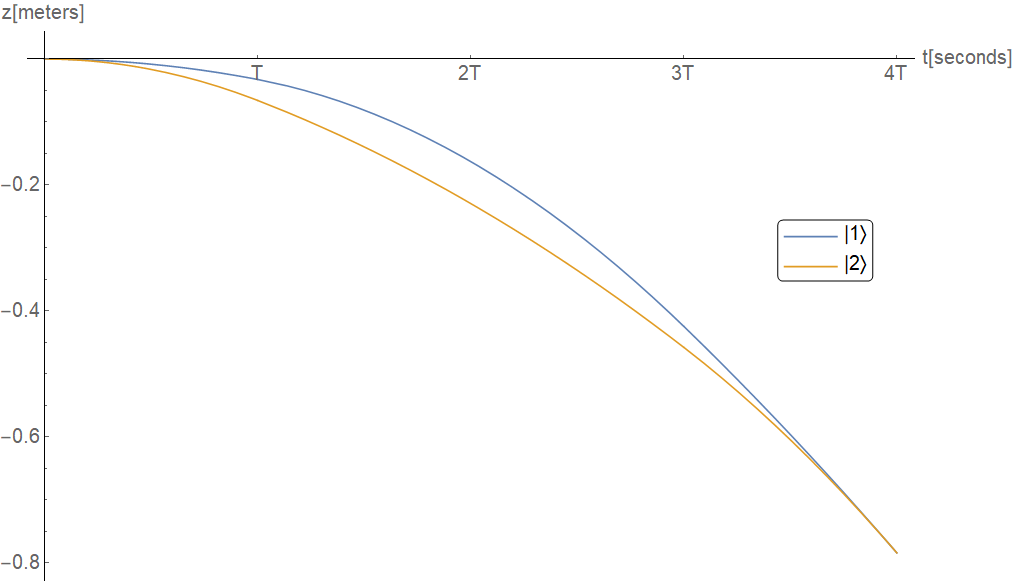
\includegraphics[width=0.8\textwidth]{posicion.png}
        \label{position_graph}
    \end{subfigure}
    \hfill
    \begin{subfigure}{1\textwidth}
        \centering
        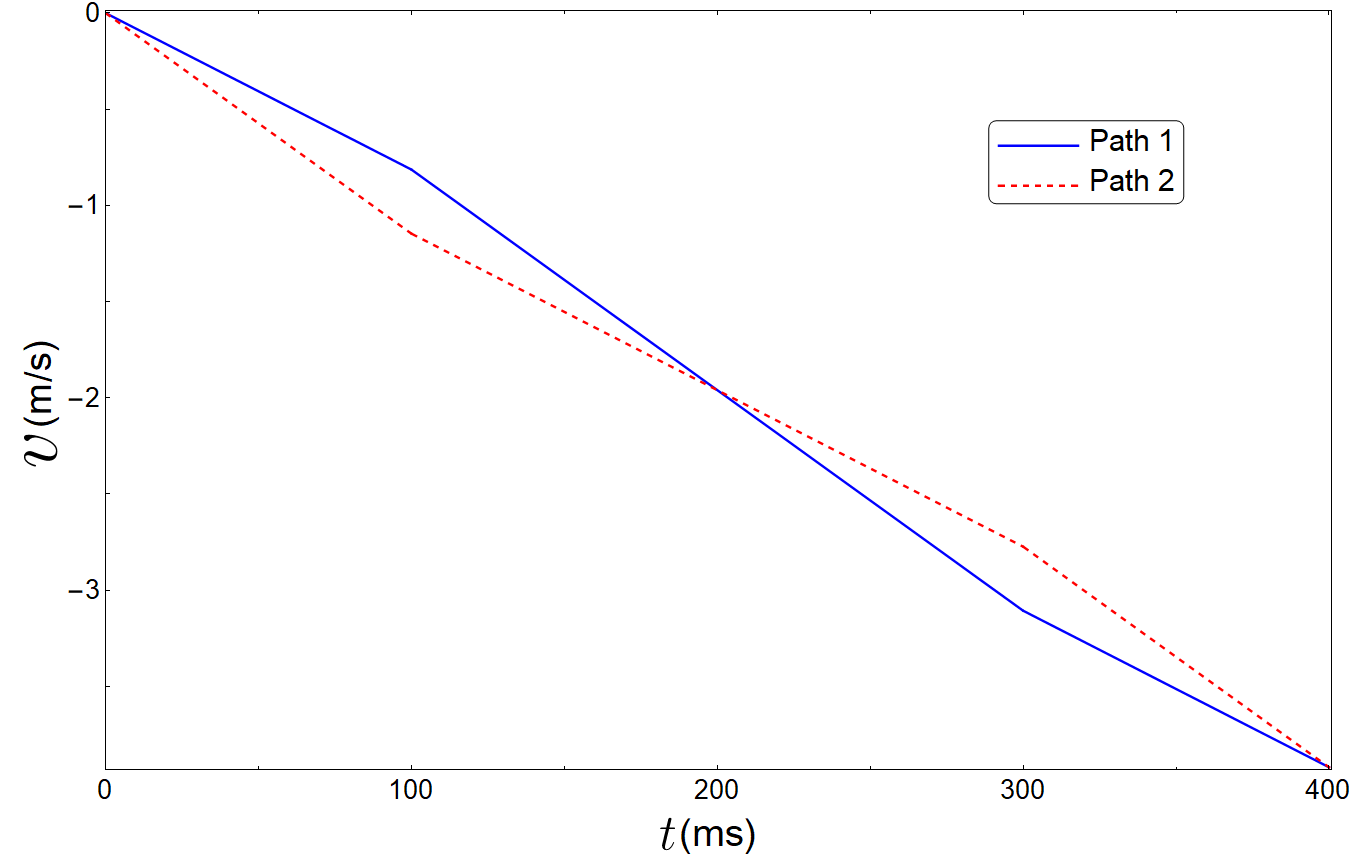
\includegraphics[width=0.8\textwidth]{velocidad.png}
        \label{velocity_graph}
    \end{subfigure}
    \caption{Position and velocity as a function of time for the two paths (blue solid and red dashed lines). We used $^{87}$Rb atoms, a gradient of $\eta = 0.05$ T/m, $T=100$ ms, $m_F=m_F'=1$ and $g_F=\pm 1/2$ for the two levels respectively.}
    \label{velocity_position_graphs}
\end{figure}

\subsubsection{Calculation of the phase signal}
Now that we have settled down the sequence of pulses needed to close the interferometer and produce interference, we are in a position to compute the expected signal for gravimetry. In the semi-classical picture, each state of the superposition follows a different path and consequently accumulates a different phase. Therefore, to obtain the gravimetry signal, we need to compute the phase accumulated by each state during the lifetime of the superposition and then compute the difference between these two phases. We compare the phase difference resulting solely from propagation\footnote{We can neglect the phase due to a difference in separation of the wave packets at the end of the interferometer since we are considering an interferometer closed in position. Additionally, we are disregarding the phase accumulation resulting from the interaction with the microwaves, as the change in momentum is negligible.} and caused by the splitting of the spatial wave function for each state. This splitting may be caused by state-dependent differences in the position, velocity (as in the case of light-pulse atom interferometers), or acceleration (as in the case of magnetic gravimetry) for the states in the superposition. The phase of each path can be computed from \cite{kasevich_light-pulse-atom-interferometry}

\begin{equation}
\label{phasepath}
\Phi_i = \frac{1}{\hbar} \int_{0}^{t} (L_{c} - E_{i}) dt',
\end{equation}
%
where $L_{c}$ is the classical Lagrangian evaluated along the classical trajectory of the i-th path and $E_{i}$ is the internal atomic energy of the atom.

Let's compute the phase difference for each of the different types of splittings described above. We suppose that all the cases begin with the atom in a single state right before the splitting. In a position splitting the atom is separated instantaneously by a distance $\Delta d=z_2-z_1$ which remains constant since the initial velocities and accelerations are the same for both states. This case would need an instantaneous recombination at the end to obtain the interference making it difficult to implement since the position splitting (or recombination) is never instantaneous \cite{quantum_brachistochrones_PhysRevX.11.011035}, and the potential required to do so introduces additional complications such as decoherence due to the shift operation in position \cite{Andreas_digital_interferometer}. For this reason, traditional atomic gravimeters, rely on velocity splitting \cite{Peters_2001} where one path has a velocity $v_0$ and the other $v_0+2 \hbar k/m$ right after the first $\pi/2$ Raman pulse. The interferometer is closed by adding a $\pi$ and a $\pi/2$ pulses. In this case, the separation grows (decreases) linearly in time for the first (second) half. On the other hand, having an acceleration splitting instead gives a separation that grows (and decreases later on) quadratically with time. The comparison of the precession of the magnetic moment in the magnetic field gradient for the two trajectories is what encodes the information about gravitational acceleration. 

From Eq. \ref{phasepath}, the phase for the splitting due to acceleration for each path turns out to be given by\footnote{We are considering a static reference frame. In this reference frame, the integral of the Lagrangian does not vanish as is the case of a reference frame that follows the atom. When using a reference frame that follows the atom, a new term that can be interpreted as the phase printed by the light on the atom arises (see for example Ref. \cite{Peters_2001}).}

\begin{equation}
\label{phasepath}
\Phi_i = \frac{m}{\hbar} \int_{0}^{t} \bigg( \frac{1}{2} v_{i}^{2}(t') - a_{\pm} z_{i}(t') - E_{i}/m \bigg) dt',
\end{equation}
%
by using the semi-classical equations of motion to solve the above integral for each interval in the sequence of pulses (Eq. \ref{pulses}), the phase difference between both paths becomes

\begin{equation}\label{finalphasediff_semiclassical}
    \Delta \Phi= \Phi_2 - \Phi_1 = 3 \frac{m}{\hbar} (a_C_{e} - a_C_{g}) \big( a_C_{e} + a_C_{g} + 2 g \big) T^{3}.
\end{equation}
%
This semi-classical result is the same as the formula originally derived for the $T^{3}$-interferometer of Ref. \cite{Zimmermann2017} (except for a factor of $3$) but was derived with much less effort.
Additionally, this result is equivalent to the phase observed in the $T^{3}$ Stern Gerlach matter wave interferometer which was proposed in Ref. \cite{SG-Interferometer-PhysRevLett.123.083601} when the delay time is set to zero (up to a constant factor in front of the magnetic gradient). The main difference between both interferometers lies in the method of producing the changes in magnetic acceleration. While the magnetic interferometer proposed here and that of Ref. \cite{Zimmermann2017} achieve changes in magnetic acceleration by changing the internal state of the atom while the magnetic gradient is kept constant in time, the SG interferometer achieves the same by using magnetic pulses that change the direction of the magnetic gradient directly without having to change the internal state of the atom. As a result, the path followed by the arms of both interferometers is the same. It is important to remark that the precision of the magnetic interferometer is not limited by the delay time imposed by electronic circuits as it is in the SG interferometer. Instead, the precision of the magnetic interferometer is primarily determined by the power of the microwaves used to change the internal state of the atom, as will be discussed later.

We can gain more insight by considering states with an opposite magnetic response, for example, the stretched states of the $\ce{^{87}_{}Rb}$ atom ($g_{F_{g, e}} = 1/2$ and $m_{F_{g, e}} = \mp 2$). In this case, the phase difference is linearly proportional to g, i.e.,

\begin{equation}\label{semi_classical_phase_example}
    \Delta \Phi_{s} = 12 \frac{\mu_{B} \eta}{ \hbar} g T^{3},
\end{equation}
where the subscript indicates that this is the total phase difference when considering the transition between the stretched states. We can compare this result with the signal measured in traditional gravimetry that uses stimulated Raman transitions to induce state transitions and changes in momentum \cite{Peters_2001}

\begin{equation}\label{traditional_gravimetry_signal}
\Delta \Phi = k_{eff} g T^2 ,
\end{equation}
%
where $\hbar k_{eff}$ is the effective momentum gained by the atom after the Raman transition has finished.

Following the same procedure used above, we can derive the phase signal for the rest of the types of splitting, including that of the light-pulse atom gravimetry (Eq. \ref{traditional_gravimetry_signal}). Table \ref{comparisonsplitting} gives the phase difference ($\Delta \Phi = \Phi_2 - \Phi_1$) for the case of splitting in position, velocity, or acceleration in terms of the total time ($T_t$) of the sequence. The sequence requires an extra $\pi$ pulse as one moves from position to velocity splitting, or from velocity to acceleration. The phase difference grows as a linear, quadratic, and cubic function of time respectively, and is proportional to the quantity responsible for the splitting. Figure \ref{phase_graph0} shows a comparison of the phase difference for the three cases as a function of the total time $T_t$. The acceleration splitting gives a bigger phase difference for a relatively short time ($T_t$) compared to the other methods. In the case of the magnetic gravimeter, $T_t$ depends on experimental parameters such as the magnetic field gradient $\eta$, and at fall times slightly below 1 s, one already gets a reasonable phase difference.

\begin{center}
\begin{table}
 \caption{\label{comparisonsplitting} Comparison of the phase difference with splitting by position, velocity, and acceleration. We suppose that the internal atomic energy of the atom in Eq. \ref{phasepath} is the same for both paths in the case of position splitting. Note that in a splitting due to differences in velocity or acceleration, the internal energy of the atom does not contribute to the phase difference since the corresponding term in the integral does not change with time and there is a change of sign due to the $\pi$-pulse(s) that cancels out the contribution for each path.}
\begin{tabular}{|l|c|c|c|} 
 \hline
 Splitting by & Position & Velocity & Acceleration \\ [0.5ex] 
 \hline
 Separated by & $\Delta d= z_2 - z_1$ & $\Delta v = v_2 - v_1$ & $\Delta a = a_2 - a_1$ , ($a_{1} = -a_{2}$) \\ 
 \hline
 Sequence & $\pi/2 \xrightarrow[]{T} \pi/2$ & $\pi/2 \xrightarrow[]{T} \pi \xrightarrow[]{T} \pi/2$ & $\pi/2 \xrightarrow[]{T} \pi \xrightarrow[]{2T} \pi \xrightarrow[]{T} \pi/2$ \\
 \hline
 Total time $T_t$ & $T_t=T$ & $T_t=2T$ & $T_t=4T$ \\
 \hline
 Phase difference $\Delta \Phi$ & $\left( \frac{mg}{\hbar} \right) \Delta d T_t$ & $\frac{1}{2} \left( \frac{mg}{\hbar} \right)$ \Delta v T_t^2& $\frac{3}{32} (\frac{m g}{\hbar}) \Delta a T_{t}^{3}$ \\ [1ex] 
 \hline
\end{tabular}
\end{table}
\end{center}

\begin{figure}
\centering
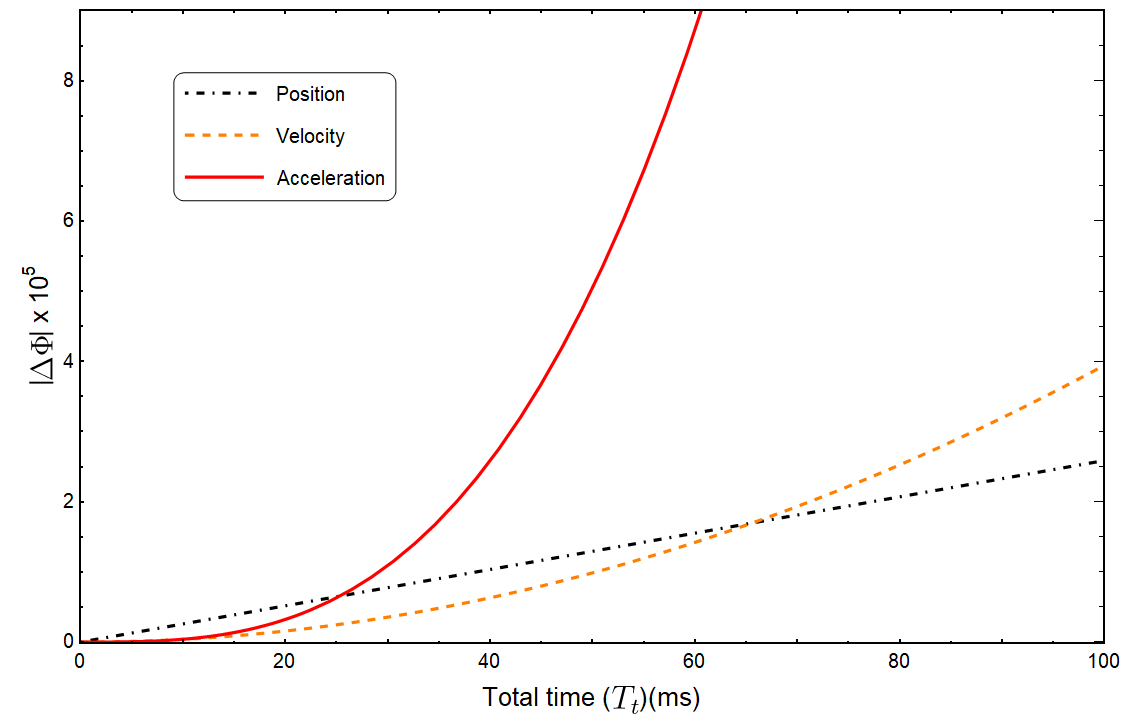
\includegraphics[width=0.9\textwidth]{comparacion_fase_posicion__velocidad_aceleracion.png}
\caption{Comparison of the phase acquired for a gravimeter separated by position (black dotted dashed line), velocity (orange dashed line), or acceleration (red solid line) as a function of the total time ($T_t$). We used $^{87}$Rb with $\Delta d = 200$ $\mu$m; $\Delta k = 2\pi /780$ nm; $\eta=0.05$ T/m, $g_{F_{g, e}} = 1/2$ and $m_{F_{g, e}} = \mp 2$.}
\label{phase_graph0}
\end{figure}

\subsection{Quantum treatment}

The calculations above considered a semi-classical picture to represent the superposition of states. Nevertheless, a correct calculation of the interferometer phase demands solving the evolution of each state using a quantum mechanical approach. A solution using time-evolution operators can be found in Ref. \cite{Zimmermann2017}. Here, we will follow a different approach. Consider an alkali-metal atom with quantized center-of-mass motion along the z-axis, subject to a constant gravitational field and interacting with a classical magnetic field of the form given by Eq. \ref{magnetic_field0} and subject to microwave excitations ($\textbf{B}_p$) that propagate along the $x$-axis with polarization along the $\hat{\textbf{q}}$-direction. Note that $\textbf{B}_p$ is only used to control the internal state of the atom, so its polarization can be chosen in any convenient direction. We focus on the $z$-axis movement of the atom since the transverse ($x$ and $y$) directions give a free evolution. The resulting Hamiltonian is \cite{Castanos2014}

\begin{equation}
\label{fullH}
H(t) = \frac{1}{2m} P_z^2 + mg Z + H_A - \boldsymbol{\mu} \cdot [\eta Z \hat{\textbf{z}} + \textbf{B}_p(t)],
\end{equation}
%
where $H_A$ is the atomic structure Hamiltonian and $\boldsymbol{\mu}$ is the magnetic dipole moment operator of the atom. The solution to this Hamiltonian, in momentum space, for the stretched states ($g_{F_{g, e}} = 1/2$ and $m_{F_{g, e}} = \mp 2$) of the $\ce{^{87}_{}Rb}$ atom is given by \cite{Castanos2014}

\begin{equation}\label{solution_momentum_space}
\widehat{\phi}(k, \tau) = \widehat{\phi}(k + q_{2}\tau, 0) \exp\left[-i q_{1} \tau + i \frac{\epsilon}{3q_{2}} k^{3} - i \frac{\epsilon}{3q_{2}} (k + q_{2} \tau)^{3} \right],
\end{equation}
%
where $k$ is the momentum of the state and $\epsilon$ is given by 

\begin{equation}\label{epsilon}
\epsilon = \frac{\hbar \kappa^{2}}{2 M \Delta W},
\end{equation}
%
where $M$ is the mass of the atom. Also, we have defined

\begin{equation}\label{q1_q2}
q_{1} = \frac{1}{2} \mathrm{,}\quad q_{2} = \bigg(\frac{M g}{\hbar \Delta W \kappa} \pm  \gamma_{1} \bigg),
\end{equation}
%
where $g_{0}$ is the acceleration of gravity and 

\begin{equation}\label{gamma_1}
\gamma_{1} = \frac{g_{s}-2 I g_{n} \frac{m_{e}}{m_{p}}}{2(g_{s}+g_{n}\frac{m_{e}}{m_{p}})},
\end{equation}
%
where $m_{e}$ and $m_{p}$ are the electron mass and the proton mass respectively and $I$ is the nuclear spin. Finally, we have defined the inverse of the characteristic length of the system as

\begin{equation}\label{kappa}
\kappa \equiv (g_{s}\frac{\mu_{B}}{\hbar} + g_{n}\frac{\mu_{n}}{\hbar}) \frac{\eta}{\Delta W} > 0,
\end{equation}
%
where $g_{s}$ is the electron spin $g$-factor, $g_{n}$ is the nuclear $g$-factor, $\mu_{B}$ is the Bohr magneton, $\mu_{n}$ is the nuclear magneton, $\hbar \Delta W$ is the field-free ground-state hyperfine splitting energy, $\eta$ is the proportionality constant of the magnetic field (Eq. \ref{magnetic_field0}), and $\tau\equiv \Delta W t$ is the non-dimensional time.

Equation \ref{solution_momentum_space} gives the evolution of the state (subject to Eq. \ref{fullH}) recursively. In particular, it gives the evolution before the pulse ($\textbf{B}_p(t) = 0$). Now, using this solution, we consider the same sequence of pulses as before (Eq. \ref{pulses}). The state at the end of the first interval will be given by

\begin{equation}\label{state_t1_momentum_space}
\widehat{\phi}_{\pm}(k, \tau) = \widehat{\phi}_{\pm}(k + q_{2_{\pm}}\tau, 0) \exp \left[-i q_{1} \tau + i \frac{\epsilon}{3q_{2_{\pm}}} k^{3} - i \frac{\epsilon}{3q_{2_{\pm}}} (k + q_{2_{\pm}} \tau)^{3} \right],
\end{equation}
%
where the subscript $\pm$ denotes the choice of either a plus or minus sign preceding $\gamma_{1}$ in the definition of $q_{2}$ (Eq. \ref{q1_q2}), i.e., it specifies the state under consideration. At the end of the second interval, the state will be given by

\begin{equation}\label{state_t2_momentum_space}
\widehat{\phi}_{\pm}(k, \tau+2\tau) = \widehat{\phi}_{\pm}(k + 2q_{2_{\mp}}\tau, \tau) \exp\left[-2i q_{1} \tau + i \frac{\epsilon}{3q_{2_{\mp}}} k^{3} - i \frac{\epsilon}{3q_{2_{\mp}}} (k + 2q_{2_{\mp}} \tau)^{3} \right],
\end{equation}
%
and at the end of the last interval, the state will be given by

\begin{equation}\label{state_t3_momentum_space}
\widehat{\phi}_{\pm}(k, \tau+2\tau+\tau) = \widehat{\phi}_{\pm}(k + q_{2_{\pm}}\tau, \tau+2\tau) \exp\left[-i q_{1} \tau + i \frac{\epsilon}{3q_{2_{\pm}}} k^{3} - i \frac{\epsilon}{3q_{2_{\pm}}} (k + q_{2_{\pm}} \tau)^{3} \right].
\end{equation}
%
We can substitute Eq. \ref{state_t2_momentum_space} into Eq. \ref{state_t3_momentum_space} to get

\begin{multline}\label{state_t3_momentum_space_2}
\widehat{\phi}_{\pm}(k, \tau+2\tau+\tau) = \widehat{\phi}_{\pm}(k + q_{2_{\pm}}\tau + 2q_{2_{\mp}}\tau, \tau)  \\ 
\exp\left[-2i q_{1} \tau + i \frac{\epsilon}{3q_{2_{\mp}}} (k+q_{2_{\pm}}\tau)^{3} - i \frac{\epsilon}{3q_{2_{\mp}}} ((k+ q_{2_{\pm}}\tau) + 2q_{2_{\mp}} \tau)^{3} \right] \\
\exp\left[-i q_{1} \tau + i \frac{\epsilon}{3q_{2_{\pm}}} k^{3} - i \frac{\epsilon}{3q_{2_{\pm}}} (k + q_{2_{\pm}} \tau)^{3} \right].
\end{multline}
%
Similarly, we can substitute Eq. \ref{state_t1_momentum_space} into the last equation to get

\begin{multline}\label{state_t3_momentum_space_final}
\widehat{\phi}_{\pm}(k, \tau+2\tau+\tau) = \widehat{\phi}_{\pm}(k + q_{2_{\pm}}\tau + 2q_{2_{\mp}}\tau + q_{2_{\pm}}\tau , 0) \\ 
\exp\left[-i q_{1} \tau + i \frac{\epsilon}{3q_{2_{\pm}}} (k+ q_{2_{\pm}}\tau + 2q_{2_{\mp}}\tau)^{3} - i \frac{\epsilon}{3q_{2_{\pm}}} ((k+q_{2_{\pm}}\tau + 2q_{2_{\mp}}\tau) + q_{2_{\pm}} \tau)^{3} \right] \\
\exp\left[-2i q_{1} \tau + i \frac{\epsilon}{3q_{2_{\mp}}} (k+q_{2_{\pm}}\tau)^{3} - i \frac{\epsilon}{3q_{2_{\mp}}} ((k+ q_{2_{\pm}}\tau) + 2q_{2_{\mp}} \tau)^{3} \right] \\
\exp\left[-i q_{1} \tau + i \frac{\epsilon}{3q_{2_{\pm}}} k^{3} - i \frac{\epsilon}{3q_{2_{\pm}}} (k + q_{2_{\pm}} \tau)^{3} \right].
\end{multline}
%
This equation describes each of the two states of the superposition at the end of the last interval and can be used to compute the total phase difference between them. Note that the first term on the right side of this equation can be interpreted as a wave packet that has not evolved in time and in consequence, it does not contribute to the phase difference. For this reason, the phase gained for each state will be given by

\begin{multline}\label{phase_momentum_space}
\widehat{\varphi}_{\pm}(k) = -4q_{1}\tau \\
+ \frac{\epsilon}{3q_{2_{\pm}}} \left[(k+ q_{2_{\pm}}\tau + 2q_{2_{\mp}}\tau)^{3} - ((k+q_{2_{\pm}}\tau + 2q_{2_{\mp}}\tau) + q_{2_{\pm}} \tau)^{3} + k^{3} - (k+q_{2_{\pm}}\tau)^{3} \right] \\
+ \frac{\epsilon}{3q_{2_{\mp}}} \left[(k+q_{2_{\pm}}\tau)^{3} - ((k+q_{2_{\pm}}\tau)+2q_{2_{\mp}}\tau)^{3} \right].
\end{multline}
%
Thereby, the total phase difference between both states when the last $\frac{\pi}{2}$-pulse is applied will be given by

\begin{equation}
\Delta \Phi = \widehat{\varphi}_{+}(k) - \widehat{\varphi}_{-}(k) = 2\left[(q_{2_{+}})^{2} - (q_{2_{-}})^{2} \right]\epsilon \tau^{3} .
\end{equation}
%
We can gain more insight into this result by substituting the definition of the non-dimensional parameters and using an approximation for the $\kappa$ and $\gamma_1$ parameters defined in Eqs. \ref{gamma_1} and \ref{kappa} as follows. The Bohr magneton and the nuclear magneton are defined as

\begin{equation}
\mu_{B} = \frac{\hbar e}{2 m_{e}} \mathrm{,}\quad \mu_{n} = \frac{\hbar e}{2 m_{p}},
\end{equation}
%
where $m_{e}$ and $m_{p}$ are the electron and proton mass respectively. However, the proton mass is several orders of magnitude larger than the electron mass, therefore, we can use the following approximation

\begin{equation}\label{kappa_approx}
\kappa \approx g_{s}\frac{\mu_{B}}{\hbar} \frac{\eta}{\Delta W}.
\end{equation}
%
Additionally, since we are considering the alkali atom of $\ce{^{87}_{}Rb}$, we have the following values for this atom \cite{KAUSHALSK1970, Bunge1993} 

\begin{equation}
g_{s} \approx 2.002 \mathrm{,}\quad g_{n} \frac{m_{e}}{m_{p}} \approx 2.002 \mathrm{,}\quad I = \frac{3}{2}.
\end{equation}
%
As a result, we can also use the following approximation

\begin{equation}\label{gamma_1_approx}
\gamma_{1} \approx 1/2.
\end{equation}
%
Thus, by using the definitions in Eqs. \ref{epsilon}-\ref{q1_q2} and the above approximations (Eqs. \ref{kappa_approx} and \ref{gamma_1_approx}), we get the total phase difference

\begin{equation}\label{quantum_gravimetry_signal_momentum_space}
\Delta \Phi = 4 \frac{\mu_{B} \eta }{\hbar} g \bigg(\frac{\tau}{\Delta W}\bigg)^{3} = 4 \frac{\mu_{B} \eta }{\hbar} g t^{3},
\end{equation}
%
where we have used $\tau\equiv \Delta W t$. Notice that, as expected, this result is the same as that obtained following a semi-classical approach (Eq. \ref{semi_classical_phase_example}) except for a factor of $3$ (see discussion following Eq. \ref{finalphasediff_semiclassical}). Therefore, the result in Eq. \ref{quantum_gravimetry_signal_momentum_space} coincides with and is a particular case of the general solution demonstrated in Ref. \cite{Zimmermann2017}

\begin{equation}\label{finalphasediff_quantum}
    \Delta \Phi= \frac{m}{\hbar} (a_{C_{e}} - a_{C_{g}}) \big( a_{C_{e}} + a_{C_{g}} + 2 g \big) T^{3}.
\end{equation}

\subsection{Detuning of the transitions due to the Zeeman effect}
We demonstrated in Eq. \ref{quantum_gravimetry_signal_momentum_space}, that it is possible to measure $g$ from the phase difference at the port of the proposed interferometer. In an ideal case, we could apply the sequence of pulses of Eq. \ref{pulses} using the correct Rabi frequencies to drive the desired transitions. However, even if we started with the correct frequency, there is a position-dependent detuning that has to be taken into account when the atoms exist in free fall. To see why, remember that the experiment takes place inside a magnetic field gradient on the z-axis of the form given by Eq. \ref{magnetic_field0} and consider transitions between two hyperfine state levels of the atom with a different magnetic quantum number

\begin{equation}\label{hyperfine_levels}
\begin{aligned}
\ket{g} = \ket{F_{g}, m_{F, g}}, \\
\ket{e} = \ket{F_{e}, m_{F, e}},
\end{aligned}
\end{equation}
%
where $m_{F, e}$($m_{F, g}$) is the magnetic quantum number of the excited(ground) state, and $F_{g}$($F_{e}$) is the total angular momentum of the excited(ground) state.
The transitions in this two-level system are characterized by a frequency  $\omega_{21}$, i.e.,

\begin{equation}
  \omega_{21} = \frac{E_{e}-E_{g}}{\hbar}.
\end{equation}
%
Since the atom is placed inside this external magnetic field, its energy levels will be split according to the (linear) Zeeman effect, i.e.,

\begin{equation}\label{linear_zeeman_eq}
  \Delta E = \mu_{B} g_{F} m_{F} B,
\end{equation}
%
where $\mu_{B}$ is the Bohr magneton and $g_{F}$ is the Landé $g_{F}$-factor. Moreover, due to the linear dependence of the magnetic field with the position, the Zeeman split will depend on the position as well, i.e.,

\begin{equation}
  \Delta E(z) = \mu_{B} g_{F} m_{F} \eta z.
\end{equation}
%
This change in the energy due to the Zeeman effect can be translated into a change in the corresponding frequency of the energy level with the magnetic number $m_{F}$ through the Planck relation, i.e.,

\begin{equation}
  \Delta \omega(z, g_{F}, m_{F}) = \frac{\mu_{B} g_{F} m_{F} \eta}{\hbar} z.
\end{equation}
%
We suppose that the wave packet describing the atom is initially located at $z_{0}$ where the magnetic field is $B_{0}$, and induce Rabi transitions between our two states by applying a perturbation with a frequency-tuned with the transition that interests us. Then, both levels will suffer a shift, so the new transition frequency will be given by 

\begin{equation}
  \omega_{21}^{\prime} = \omega_{21} + \Delta \omega(z_{0}, g_{F_{e}}, m_{F_{e}}) -  \Delta \omega(z_{0}, g_{F_{g}}, m_{F_{g}}) =  \omega_{21} + \frac{\mu_{B} g_{F_{eff}} m_{F_{eff}} \eta}{\hbar} z_{0},
\end{equation}
%
where we have defined an effective product between the quantum magnetic numbers and the Landé $g_{F}$-factors as

\begin{equation}\label{detuning}
    g_{F_{eff}} m_{F_{eff}} \equiv g_{F_{e}} m_{F_{e}} - g_{F_{g}} m_{F_{g}}.
\end{equation}
%
Hence, the detuning of the Rabi oscillations when the atom is at $z$ will be given by

\begin{equation}\label{detunig_atom_width}
  \delta (z) = \omega_{B} - \omega_{21}^{\prime} = \frac{\mu_{B} g_{F_{eff}} m_{F_{eff}} \eta}{\hbar} (z-z_{0}).
\end{equation}

\subsection{The warning width}
It turns out that this detuning in Eq. \ref{detunig_atom_width} sets a constraint in the width, in position space, that the atom's wave function can have to have resonant transitions. To determine this warning width, we recall that the probability of finding the atom in the excited state at time $t$ when it was initially in the ground state at $t=0$ is given by \cite{sakurai2017modern}

\begin{equation}\label{rabi_oscillations_exact}
  |c_{e}(t)|^{2} =\frac{\Omega^{2}}{\tilde{\Omega}^{2}} \sin^{2}\bigg[\frac{\tilde{\Omega} t}{2} \bigg],
\end{equation}
%
where $\tilde{\Omega}$ is defined in terms of the Rabi flopping frequency $\Omega$ and the detuning $\delta$\footnote{Other references name $\tilde{\Omega}$ as the Rabi flopping frequency instead of $\Omega$. In any case, notice that $\tilde{\Omega}$ is the parameter that contains the information about the transition frequency while $\Omega$ only contains the information about the strength of the electromagnetic field.}, i.e.,

\begin{equation}\label{omega_tilde_definition}
  \tilde{\Omega} = \sqrt{\delta^{2} + \Omega^{2}}.
\end{equation}
%
Now, consider the point where a $\pi$-pulse results in no transfer of population, i.e., 

\begin{equation}\label{detuning_condition}
\sqrt{\big[ \delta (z) \big]^{2} + \Omega^{2}} \bigg( \frac{t}{2} \bigg) = \pi,
\end{equation}
%
from which we get

\begin{equation}\label{detuning_at_zhwm}
\delta (z) = \frac{\sqrt{4 \pi^{2} - \Omega^{2} t^{2}}}{t}.
\end{equation}
%
Using the above result and Eq. \ref{detuning}, we get

\begin{equation}\label{width_set_by_detuning}
\Delta Z = \frac{\sqrt{4 \pi^{2} - \Omega^{2} t^{2}}}{t} \frac{\hbar}{\mu_{B} g_{F_{eff}} m_{F_{eff}} \eta}.
\end{equation}
%
For experimental purposes, we would like to have $\Omega$ fixed. Therefore, the width will be fixed by $t$. For example, if we use a $\pi$-pulse, i.e., $t=\pi/\Omega$. Then, the warning width will be given by

\begin{equation}\label{warning_width}
\Delta Z = \pi \sqrt{3} \Omega \frac{\hbar}{\mu_{B} g_{F_{eff}} m_{F_{eff}} \eta}.
\end{equation}
%
Thus, to stay in resonance during the application of the Rabi pulses, the width of the atom's wave function in position space must remain smaller than the width given by Eq. \ref{warning_width}.

Finally, notice that usually the electric field dominates since it is several orders of magnitude larger than the magnetic field so the Rabi flopping frequency is usually taken to be

\begin{equation*}
\Omega = \frac{- e E_{0} \bra{e} r \ket{g}}{\hbar},
\end{equation*}
%
where $r$ is the position operator in the direction of the polarization of the electric field, $E_{0}$ is the amplitude of the electric field, and $e$ is the electron charge. Nonetheless, for an alkali atom inside a magnetic field gradient, the transitions are driven by the magnetic field of the microwaves and not by the electric field. This is because we will only consider transitions between hyperfine sub-levels in the ground state $5^{2}S_{1/2}$ of $\ce{^{87}_{}Rb}$ \cite{Castanos2014} for which the dipole matrix elements are zero due to selection rules \cite{Steck2010}. Therefore, the Rabi flopping frequency will depend solely on the magnetic field, i.e.,\footnote{This is the paramagnetic contribution to the magnetic moment of the atom and is valid for weak magnetic fields. In general, there is another quadratic contribution called the diamagnetic moment of the atom which is very small \cite{scotto2016}.}

\begin{equation}\label{rabi_frequency_magnetic_field}
\Omega = \frac{- B_{0} \bra{e} \mu \ket{g}}{\hbar},
\end{equation}
%
where $\mu$ is the total magnetic moment operator in the direction of the polarization of the magnetic field, $B_{0}$ is the amplitude of the magnetic field $\textbf{B}$ which in the case of a monochromatic polarized microwave can be written in the generic form

\begin{equation}
    \textbf{B} =  B_{0} \cos(\omega t) \boldsymbol{\hat{e}},
\end{equation}
%
where we have ignored the spatial variation due to the dimensions of the atom. Thereby, the amplitude of the magnetic field will set the warning width. The more intense the magnetic field, the larger the warning width and vice-versa.

\subsection{Expansion of the atomic wave function for a pure state}
As previously seen, to have resonant transitions, the width of the atom's wave function in position space has to be smaller than the warning width set by Eq. \ref{warning_width}. Therefore, it is imperative to know what is the width of the wave packet and its expansion. In general, the expansion will depend on how the initial state was prepared and its initial width. In this section, we will consider the case of a pure state resulting from the application of a selector pulse in position space and later, we will consider the case where the expansion is described by the evolution of a thermal ensemble of atoms initially trapped in an optical dipole trap. We will begin by reviewing the time evolution of a Gaussian wave packet.

\subsubsection{Time-evolution of the free wave packet}
We begin by considering a superposition of plane waves with different amplitudes \cite{gasiorowicz2003quantum}

\begin{equation}\label{free_wave_packet_momentum_space_integral}
    \Psi (z, t) =  \int_{- \infty}^{\infty} dk A(k) e^{i (kz-\omega t)} ,
\end{equation}
%
where $k$ is the wave number and the amplitude $A(k)$ is of the Gaussian form

\begin{equation}\label{gaussian_amplitude_free_wave_packet}
    A(k) = C e^{-\alpha(k-k_{0})^{2}/2} ,
\end{equation}
%
where $k_{0}$ is the center of the distribution, $C$ is a scale factor that we can use to normalize the wave packet, and $\alpha$ is a parameter that defines the initial width of the wave packet as we will see in a moment. To compute the integral in Eq. \ref{free_wave_packet_momentum_space_integral}, we need to establish the dependence between $\omega$ and $k$, i.e., the dispersion relation. We will consider the dispersion relation to be sharply peaked about $k=k_{0}$ and use a Taylor expansion about this point to second order, i.e.,

\begin{equation}\label{dispersion_relation_free_wave_packet}
    \omega(k) = \omega_{0} + (k-k_{0})\upsilon_{g} + \frac{1}{2}(k-k_{0})^{2} \beta ,
\end{equation}
%
where $\omega_{0}=\omega(k_{0})$, and $\upsilon_{g}$ is the group velocity defined as

\begin{equation}
    \upsilon_{g} \equiv \bigg(\frac{\partial \omega(k)}{\partial k}\bigg)_{k=k_{0}},
\end{equation}
%
and $\beta$ is given by

\begin{equation}
    \beta \equiv \bigg(\frac{\partial^2 \omega(k)}{\partial k^2}\bigg)_{k=k_{0}}.
\end{equation}
%
Now, we can substitute Eqs. \ref{gaussian_amplitude_free_wave_packet}-\ref{dispersion_relation_free_wave_packet} into Eq. \ref{free_wave_packet_momentum_space_integral} and workout the integral. Then, the wave packet in position space, normalized and initially centered around $z_{0}$, is given by

\begin{equation}
    \Psi (z, t) = \bigg(\frac{\sqrt{\alpha}}{2 \pi ^{3/2}} \bigg)^{1/2} \sqrt{\frac{2 \pi}{\alpha + i \beta t}} \exp \left[{\frac{i}{2}\frac{(z - z_{0} - \upsilon_{g} t)^{2}}{\beta t - i \alpha}} \right]  \exp[{i (k_{0}(z-z_{0})-\omega_{0} t)}].
\end{equation}
%
We can cast the above equation into a more illuminating form by putting the complex factors in the denominators in the standard form ($Z = [\Re(Z)+i\Im(Z)]$), and by using the de Moivre's theorem to compute the required squared root. In this way, we obtain the expansion of the free Gaussian wave packet as follows

\begin{multline}\label{free_wave_packet_position_space_centered_0} 
    \Psi (z, t) = (2\pi)^{-1/4} \bigg(\frac{\alpha^{2} + \beta^{2} t^{2}}{2\alpha}\bigg)^{-1/4} \exp \left[-\frac{1}{4} \frac{ (z - z_{0} - \upsilon_{g} t)^{2}}{(\alpha^{2} + \beta^{2}t^{2})/(2\alpha)}  \right] \\ \exp \left[i \bigg(k_{0}(z-z_{0}) - w_{0}t + \frac{\beta t}{2}\frac{(z - z_{0} - \upsilon_{g} t)^{2}}{\alpha^{2} + \beta^{2}t^{2}} - \frac{1}{2} \arctan\bigg[\frac{\beta t}{\alpha}\bigg]\bigg) \right].
\end{multline}
%
If we re-accommodate terms, we can write the equation describing the evolution of the normalized free wave packet as

\begin{multline}\label{free_wave_packet_position_space_centered_z0_final_form}
    \Psi (z, t) = \left[\frac{1}{2 \pi \big(\sigma_{z}(t)\big)^2} \right]^{1/4} \exp \left[-\frac{1}{4} \frac{ \big(z - z_{0} - \upsilon_{g} t \big)^{2}}{\big(\sigma_{z}(t)\big)^{2}} \right] \exp \left[-\frac{i}{2} \arctan\Bigg(\frac{\beta t }{2\big(\sigma_{z}(0)\big)^{2}}\Bigg) \right] \\ \exp \left[i \bigg(k_{0}(z-z_{0}) - w_{0}t + \frac{\big[(z - z_{0})^{2} + 2 z_{0} \upsilon_{g} t \big]}{ 4[\sigma_{z}(t)\sigma_{z}(0)]^{2}} \frac{\beta t}{2} + \frac{\upsilon_{g} t (\upsilon_{g} t - 2z)}{4[\sigma_{z}(t)\sigma_{z}(0)]^{2}} \frac{\beta t}{2} \bigg) \right],
\end{multline}
%
where the width of the wave packet is given by

\begin{equation}
\sigma_{z}(t) = \sqrt{\frac{\alpha^{2} + \beta^{2}t^{2}}{2 \alpha}}.
\end{equation}
%
Thereby, the initial width of the free wave packet is given by

\begin{equation}
\sigma_{z}(0) = \sqrt{\alpha / 2}.
\end{equation}
%
Hence, the expansion of the free wave packet is described by 

\begin{equation}\label{free_wave_packet_width} 
\sigma_{z}(t) = \sqrt{[\sigma_{z}(0)]^{2} + \left[\frac{\beta t}{2 \sigma_{z}(0)} \right]^{2}}.
\end{equation}

\subsubsection{Initialization of the free wave packet}
Notice that we can take advantage of the result in Eq. \ref{warning_width} to perform a measurement in position space and discard the atoms that did not end up in the desired final state because the width of its wave function was larger than $\Delta Z$, so we end up with a cloud of atoms with a definite uncertainty (width) in position space. We can use this selector pulse to set the initial width of the atom's wave function in position space. This approach only works if the initial width of the atom's wave packet is larger than the warning width set according to Eq. \ref{width_set_by_detuning}. The application of this selector pulse results approximately in a pure state (for the external degrees of freedom) described by a Gaussian wave packet of the form given by Eq. \ref{free_wave_packet_position_space_centered_z0_final_form} with its expansion described by Eq. \ref{free_wave_packet_width}. Notice that if the initial width is too small, the wave packet will expand quickly and the detuning will begin to be a problem. On the other hand, if the initial width is too large, the expansion time will be short. It seems that there should exist a sweet spot where the initial width is not too small or too big. Thus, we need to try to optimize Eq. \ref{free_wave_packet_width}. As mentioned earlier, the maximum Rabi frequency that can be obtained in the laboratory will usually set the final width that can be used to drive the transitions, thus, it makes sense to set the final width as a constant in Eq. \ref{free_wave_packet_width} and find out the initial width that maximizes the time needed to reach the final width. Thereby, we re-write Eq. \ref{free_wave_packet_width} as follows

\begin{equation}\label{expansion_wave_packet_time_solution}
    t = 2 \frac{\sigma_{z0}}{\beta} \sqrt{(\sigma_{zf})^2 - (\sigma_{z0})^2},
\end{equation}
%
where $\sigma_{z0}$ and $\sigma_{zf}$ are the initial and final width respectively. The initial width that maximizes this expression is given by

\begin{equation}\label{ratio_optimial_initial_width_vs_final_width_time_max}
    (\sigma_{z0})^{\ast} = \frac{\sigma_{zf}}{\sqrt{2}}.
\end{equation}
%
If we substitute back this value into Eq. \ref{expansion_wave_packet_time_solution}, we get the time that we can let the wave packet expand

\begin{equation}\label{t_maximized_given_initial_width}
    t_{max} = \frac{\sigma_{zf} ^ 2}{\beta}.
\end{equation}
%
By comparing Eq. \ref{free_wave_packet_position_space_centered_z0_final_form} and the wave function of Eq. \ref{solution_momentum_space} written in position space for an initial coherent state wave packet \cite{Castanos2014}, we get that $\beta = \hbar / M$ where $M$ is the mass of the atom. We show in Fig. \ref{optimization_expansion_width} the optimization of the wave packet for a given final width.

\begin{figure}
\centering
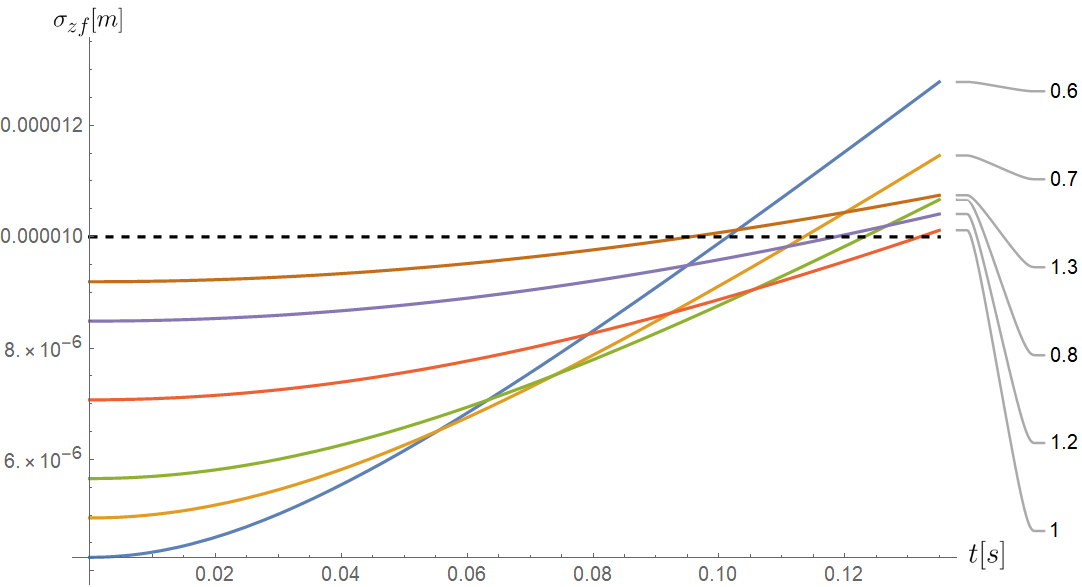
\includegraphics[width=0.9\textwidth]{maximize_expansion_time.png}
\caption{Maximization of the time needed to reach a given final width  $\sigma_{z0}$. The initial width $(\sigma_{z0})^{\ast}$ that maximizes the time needed to reach $\sigma_{zf}$ is given in Eq. \ref{ratio_optimial_initial_width_vs_final_width_time_max}. The numbers on the right mean: $times$ $(\sigma_{z0})^{\ast}$; so $0.6$ means $0.6(\sigma_{z0})^{\ast}$, $0.7$ means $0.7(\sigma_{z0})^{\ast}$, and so on. The dashed line represents the desired final width $\sigma_{zf}$. This plot was generated by considering $M$ in Eq. \ref{t_maximized_given_initial_width} equal to the mass of the $\ce{^{87}_{}Rb}$ atom.}
\label{optimization_expansion_width}
\end{figure}

\subsection{Expansion of the atomic cloud for an ensemble of atoms initially trapped in thermal equilibrium}
The pure state considered in the last section, helped us to understand the general behavior of the expansion of the wave function. However, it does not take into consideration the thermal distribution of the atoms. To take into account the effect of the temperature, we need to consider the density matrix of the ensemble of atoms. Thus, in a more realistic computation, the expansion of the wave packet has to depend on both the temperature of the atomic cloud and the frequency of oscillation of the atoms in the initial trap.

\subsubsection{Initial Conditions of the atomic cloud}
The first step in atomic gravimetry is to trap and cool the atoms to be used. Let us assume that we use an optical dipole trap and that the atoms in this trap oscillate along the z-axis under a harmonic oscillator potential with frequency $\omega$. Furthermore, let's suppose that we keep the atoms trapped until they reach a thermal equilibrium\footnote{The conditions to get a thermal equilibrium will depend on the type of trap chosen.}. Afterward, we turn off the trap and let the cloud of atoms expand. After we release the atoms from the trap, every atom will have a different wave function so we will have to rely on statistical methods to know the properties of this ensemble. In the following sections, we will give a brief review of the formalism of the density matrix and show how the density matrix for our particular case can be computed. We will suppose that the ensemble is a canonical ensemble kept at temperature $T$ even after we release them from the trap. This is justified because the potential is turned off instantaneously so we can expect that the thermal equilibrium stands for a short period since the atoms do not have enough time to reach the walls of the system to interchange kinetic energy. Besides, we suppose that we have a dilute gas so the atoms do not interact with each other. Finally, it is important to mention that for the next results, we will consider that this ensemble follows the Boltzmann statistics. This is justified since trapping atoms by simply using an optical dipole trap is not enough to produce a Bose-Einstein condensate. To achieve the quantum regime of Bose-Einstein statistics, we would need to additionally use evaporative cooling.

\subsubsection{Review of the density matrix}
If we wish to compute statistic properties for our ensemble, we need to compute the density matrix. The density matrix for non-degenerate states is defined as

\begin{equation}
    \rho = \sum_{n} w_{n} \ket{\phi_n} \bra{\phi_n},
\end{equation}
%
where the probability $w_{n}$ is normalized such that $\sum_{n} w_{n} = 1$. In the case where $\ket{\phi_n}$ are the eigenvectors of the Hamiltonian $H$, i.e., $H \ket{\phi_n} = E_n \ket{\phi_n}$, we have that \cite{sakurai2017modern}

\begin{equation}
    w_{n} = e^{-\beta E_{n}} / Q,
\end{equation}
%
where $w_{n}$ is the probability of finding, in the ensemble, a system with energy $E_{n}$, i.e., in the state $\ket{\phi_n}$.
Also, $Q = \sum_{n} e^{-\beta E_{n}}$ is the well-known partition function, and $\beta = \frac{1}{k T}$, where k is the Boltzmann constant and $T$ is the temperature of every system in the ensemble. Therefore, we have that

\begin{equation}
    \begin{split}
        \rho & = Q^{-1} \sum_{n} e^{-\beta H} \ket{\phi_n} \bra{\phi_n} = Q^{-1} e^{-\beta H} \sum_{n} \ket{\phi_n} \bra{\phi_n}, \\ & = \frac{e^{-\beta H}}{Tr(e^{-\beta H})}, \\ & = Q^{-1} e^{-\beta H}.
    \end{split}
\end{equation}
%
Now, we will try to compute the density matrix by following the method described in \cite{Feynman1972-tl}. Let us define the non-normalized density matrix $\rho_u$ given by

\begin{equation}
    \rho_u \equiv e^{-\beta H}.
\end{equation}
%
If we take the derivative of this equation with respect to $\beta$, we have

\begin{equation}\label{bloch_eq}
    - \frac{\partial \rho_u}{\partial \beta} = H \rho_u.
\end{equation}
%
Thereby, by solving this PDF we can find find $\rho_u$. The initial condition needed to solve this equation is that if we take the limit $\beta \longrightarrow 0$, i.e., $T \longrightarrow \infty$, we have to recover the density matrix of a completely random ensemble, that is

\begin{equation}\label{bloch_eq_initial_cond}
    \rho_u(0) = 1.
\end{equation}
%
From now on, we will omit the sub-index and just write $\rho$ for the non-normalized density matrix. What's more, to write the matrix elements in position space, we will use the following notation

\begin{equation}
    \bra{x} \rho \ket{x'} \equiv \rho(x, x' | \beta) = \sum_{n} Q^{-1} e^{\beta E_{n}} \phi_n (x) \phi_{n}^{*} (x').
\end{equation}
%
Therefore, in position space, Eqs. \ref{bloch_eq} and \ref{bloch_eq_initial_cond} have the following form

\begin{equation}\label{bloch_eq_pos_space}
    - \frac{\partial \rho(x, x' | \beta)}{\partial \beta} = H_{x} \rho(x, x' | \beta),
\end{equation}
%
and

\begin{equation}\label{bloch_eq_initial_cond_pos_space}
    \rho(x, x' | 0) = \delta(x-x').
\end{equation}
%
Note that $H_{x}$ operates in the $x$-axis. Let us see how to solve these equations for different Hamiltonians.

\paragraph{Density matrix for a 1-D free particle Hamiltonian}
Now, we will show how to solve Eqs. \ref{bloch_eq_pos_space} and \ref{bloch_eq_initial_cond_pos_space} for the case of the 1-dimensional free particle Hamiltonian, i.e.,

\begin{equation}
    H = \frac{\hat{p}^{2}}{2m},
\end{equation}
%
where $\hat{p}$ is the momentum operator given by

\begin{equation}
    \hat{p} = -i\hbar \nabla.
\end{equation}
%
Therefore, the equations to solve are

\begin{equation}
    - \frac{\partial \rho(x, x' | \beta)}{\partial \beta} = -\frac{\hbar^{2}}{2m} \frac{\partial^{2}}{\partial x^{2}} \rho(x, x' | \beta),
\end{equation}
%
and

\begin{equation}
    \rho(x, x' | 0) = \delta(x-x').
\end{equation}
%
The solution that satisfies these equations can be easily found to be

\begin{equation}
    \rho(x, x' | \beta) = \sqrt{\frac{m}{2\pi \hbar^{2} \beta}} \exp\bigg[-\bigg(\frac{m}{2 \hbar^{2} \beta}\bigg)(x-x')^{2}\bigg].
\end{equation}
%
This is the equation of a normal distribution and can be written as

\begin{equation}\label{density_matrix_free_particle}
    \rho(x, x' | \beta) = \frac{1}{\sigma \sqrt{2\pi}}\exp\bigg[-\frac{1}{2} \frac{(x-x')^{2}}{\sigma^{2}} \bigg],
\end{equation}
%
where the standard deviation of the distribution is given by

\begin{equation}\label{free_particle_density_mat}
    \sigma = \hbar \sqrt{\frac{\beta}{m}}.
\end{equation}
%
This result means that the matrix elements of the density operator in position space follow a normal distribution centered at the diagonal. Then, the diagonal elements are given by

\begin{equation}\label{free_particle_density_mat_diagonal}
    \rho(x, x | \beta) = \frac{1}{\sigma \sqrt{2\pi}}.
\end{equation}
%
Observe that this solution is not normalizable. This makes sense since the wave function of a free particle is not normalizable either.

\paragraph{Density matrix for an ensemble of free particles in a box}
If we have an ensemble of free particles confined in a box, the matrix elements of the density operator are still given by Eqs. \ref{free_particle_density_mat} and \ref{free_particle_density_mat_diagonal}. However, this time the diagonal elements are normalizable. If the box (1-dimensional) has a length $L$, we have that the normalization constant is given by

\begin{equation}
   \begin{split}
        N & = \int_{-L/2}^{L/2} \rho(x, x | \beta) dx, \\ & = \frac{1}{\sigma \sqrt{2\pi}} \int_{-L/2}^{L/2} dx, \\ & = \frac{L}{\sigma \sqrt{2\pi}.}
   \end{split}
\end{equation}

\subsubsection{Density matrix for an ensemble of atoms subjected to a harmonic oscillator potential}
Notice that the potential in an optical dipole trap can be approximated with a harmonic oscillator \cite{Metcalf1999}. Thus, now, we focus on solving Eqs. \ref{bloch_eq_pos_space} and \ref{bloch_eq_initial_cond_pos_space} for the case of a harmonic oscillator Hamiltonian, i.e.,

\begin{equation}
    H = \frac{\hat{p}^{2}}{2m} + \frac{m \omega^{2} \hat{x}^{2}}{2}.
\end{equation}
%
With this Hamiltonian, the equation to be solved becomes

\begin{equation}\label{oscillator_pde}
    -\frac{\partial \rho}{\partial \theta} = -\frac{\partial^{2} \rho}{\partial \xi^{2}} + \xi^{2}\rho,
\end{equation}
%
where we have introduced the non-dimensional quantities

\begin{equation}
    \xi \equiv \sqrt{\frac{m \omega}{\hbar}} x,
\end{equation}
%
and

\begin{equation}
    \theta \equiv \frac{\hbar \omega}{2} \beta.
\end{equation}
%
Similarly, the initial condition can be re-written using the non-dimensional variable $\xi$ and by using the composition property of the Dirac delta function

\begin{equation}
    \delta[f(x)] = \sum_{i}\frac{1}{|f'(x_{i})|} \delta(x-x_{i}),
\end{equation}
%
where $f(x_{i})=0$ and $f'(x_i)\neq0$. Thus, if we write

\begin{equation}
    f(x)=\xi-\xi'=\sqrt{\frac{m\omega}{\hbar}}(x-x'),
\end{equation}
%
we get

\begin{equation}
    \delta[f(x)] = \delta(\xi-\xi')=\sqrt{\frac{\hbar}{m\omega}}\delta(x-x'),
\end{equation}
%
and the initial condition can be written as

\begin{equation}\label{oscillator_pde_initial_condition}
    \rho(\xi,\xi'|0) = \sqrt{\frac{m\omega}{\hbar}} \delta(\xi-\xi').
\end{equation}
%
In order to solve Eq. \ref{oscillator_pde}, we will analyze the solution in the high-temperature limit, i.e., when $\theta \longrightarrow 0$. In this limit, the particles have to behave like a free particle so the solution has to be the Gaussian distribution in Eq. \ref{density_matrix_free_particle}. Thus, we suppose a solution of the form

\begin{equation}\label{oscillator_pre_solution}
    \rho = exp\big[-\big(a(\theta)\xi^{2} + b(\theta)\xi + c(\theta)\big)\big],
\end{equation}
%
where $a$, $b$, and $c$ are parameters that depend on $\theta$. If we differentiate this equation and substitute it back into Eq. \ref{oscillator_pde}, we reduce the PDE into the following system of ordinary differential equations

\begin{equation}\label{oscillator_system_ode}
    \begin{split}
        \frac{d a}{d\theta} = 1 - 4a^{2}, \\ \frac{d b}{d\theta}=-4ab, \\ \frac{dc}{d\theta}=2a-b^{2}.
    \end{split}
\end{equation}
%
The first of these equations has two possible solutions,

\begin{equation}
    a = \frac{1}{2} \coth\big(2(\theta - c_{1})\big),
\end{equation}
%
and 

\begin{equation}
    a = \frac{1}{2} \tanh\big(2(\theta - c_{1})\big),
\end{equation}
%
where $c_{1}$ is a constant.
However, if we want to satisfy the initial condition, we have to choose the first solution. Then, we substitute this solution back into the second line of Eq. \ref{oscillator_system_ode}, and solve the resulting ODE to get

\begin{equation}
    b = c_{2} \coth \big( 2(\theta - c_{1}) \big) \sech \big( 2(\theta - c_{1}) \big),
\end{equation}
%
where $c_{2}$ is a constant. Similarly, if we substitute this solution and the solution for $a$ into the last line of Eq. \ref{oscillator_system_ode}, and solve the resulting ODE, we get

\begin{equation}
    c = \frac{1}{2} \ln \Big(\sinh \big( 2(\theta - c_{1}) \big) \Big) + \frac{c_{2}^{2}}{2} \coth \big( 2(\theta - c_{1}) \big) - \ln (c_{3}),
\end{equation}
%
where $c_{3}$ is a constant. Then, we can substitute back the solutions for Eq. \ref{oscillator_system_ode} into Eq. \ref{oscillator_pre_solution} to get

\begin{equation}
    \rho = \frac{c_{3}}{\sqrt{\sinh(2\theta)}} \exp \bigg[ -\coth \big(2(\theta - c_{1})) \bigg( \frac{\xi^{2}}{2} + c_{2} \sech \big( 2(\theta - c_{1}) \big)\xi + \frac{c_{2}^{2}}{2} \bigg) \bigg]. 
\end{equation}
%
Nonetheless, to satisfy the initial condition (Eq. \ref{oscillator_pde_initial_condition}), we have to choose $c_{1}=0$, so we have

\begin{equation}
    \rho = \frac{c_{3}}{\sqrt{\sinh(2\theta)}} \exp \bigg[ -\coth \big(2\theta) \bigg( \frac{\xi^{2}}{2} + c_{2} \sech \big( 2\theta \big)\xi + \frac{c_{2}^{2}}{2} \bigg) \bigg]. 
\end{equation}
%
Now, we have to analyze the behavior of our solution in the high-temperature limit, i.e., $\theta \longrightarrow 0$. For that reason, we use the following Taylor expansions

\begin{equation}
    \begin{split}
        \sinh x = x + \frac{x^{3}}{16} + \cdots, \\ \coth x = \frac{1}{x} + \frac{x}{3} + \cdots, \\ \sech x = 1 - \frac{x^{2}}{2} + \cdots.
    \end{split}
\end{equation}
%
Then, if we expand at first order the trigonometric functions in the solution for $\rho$, we get

\begin{equation}
    \rho = \frac{c_{3}}{\sqrt{2\theta}} \exp \big[ -\frac{1}{4\theta}(\xi^{2} + 2c_{2}\xi + c_{2}^{2}) \big].
\end{equation}
%
Thus, if we choose $c_{2}=-\xi'$ to complete the square in the exponential, and $c_{3} = \sqrt{\frac{m\omega}{2\pi \hbar}}$, we recover the solution for the free particle (Eq. \ref{density_matrix_free_particle}) as expected. Therefore, the desired solution for the harmonic oscillator potential is

\begin{equation}\label{harmonic_osc_density_matrix}
    \rho(\xi, \xi'|\beta) = \sqrt{\frac{m\omega}{2\pi \hbar \sinh(2\theta)}} \exp \Bigg[ -\frac{\coth(2\theta)}{2} \big( \xi^{2} - 2\xi' \xi \sech(2\theta) + \xi'^{2} \big) \Big].
\end{equation}
%
Note that when $\theta \approx 0$, we recover the initial condition, i.e.,

\begin{equation}
    \rho(x, x' | \beta) \approx \sqrt{\frac{m\omega}{2\pi\hbar (2\theta)}} \exp \bigg(- \frac{m\omega}{2\hbar} \frac{(x-x')^{2}}{2\theta} \bigg) \xrightarrow{\theta \longrightarrow 0} \delta(x-x'),
\end{equation}
%
where we have used the fact that

\begin{equation}
    \lim_{a \to 0^{+}} \sqrt{\frac{1}{\pi a}} \exp \bigg(\frac{-(x-x_{0})^{2}}{a} \bigg) = \delta(x-x_{0}).
\end{equation}
%
Note that since the partition function is defined as the trace of the density operator, we will only need the diagonal elements to compute average values\footnote{It can be easily shown that the partition function is the trace of the density operator if we use the energy eigenkets. However, when two matrices are similar, their trace is the same, independently of the basis chosen, so this result is general.}. Fortunately, the diagonal elements of the density operator can be written in a very simple form by using the following trigonometric identity

\begin{equation}
    \coth (2\theta) \big[1-\sech(2\theta) \big] = \tanh\theta.
\end{equation}
%
Therefore, for the diagonal elements of the density operator, we have 

\begin{equation}
    \rho(x,x|\beta) = \sqrt{\frac{m\omega}{2\pi\hbar\sinh(2\theta)}} \exp \bigg( -\frac{m\omega}{\hbar}x^{2} \tanh(\theta) \bigg).
\end{equation}
%
Thus, we can compute the average value of the squared position as follows

\begin{equation}
    \overline{x^{2}} = \frac{\int x^{2} \rho(x,x|\beta) dx}{\int \rho(x,x|\beta) dx} = \frac{\hbar}{2m\omega} \coth\bigg( \frac{\omega\beta\hbar}{2} \bigg).
\end{equation}
%
Notice that we had to normalize the result because the density operator was not normalized. Similarly, for the average of the position, we have

\begin{equation}
    \overline{x} = \frac{\int x \rho(x,x|\beta) dx}{\int \rho(x,x|\beta) dx} = 0.
\end{equation}
%
Therefore, the dispersion of the distribution function in position space can be easily computed as follows

\begin{equation}\label{dispersion_harmonic_oscillator}
    \sigma_{x}^{2} = \overline{x^{2}} - \overline{x}^{2} = \frac{\hbar}{2m\omega} \coth \bigg( \frac{\hbar\omega}{2kT} \bigg).
\end{equation}
%
In the case of $\ce{^{87}_{}Rb}$ atoms, we have $m\approx1.4*10^{-25}$ Kg. Besides, a typical temperature value for an atomic trap is $T\approx 1 \mu$K, while a typical frequency value is $\omega = 2\pi *10$kHz. With these values, the width of the distribution function in position space becomes

\begin{equation}
    \sigma_{x} \approx 0.1 \mu m.
\end{equation}

\subsubsection{Time-evolution of the density matrix}
The calculation of the last section was for the static case where the density matrix does not change in time. Nevertheless, once the atoms are released from the atomic trap, we can expect the density matrix to evolve in time under a new Hamiltonian. Thus, we need to compute the evolution of the density operator. Let's consider that at time $t_{0}$ the density operator is given by

\begin{equation}
    \rho(t_{0}) = \sum_{n} \omega_{n} \ket{n(t_{0})}\bra{n(t_{0})}.
\end{equation}
%
In the Schrodinger picture, the state vectors evolve in time using the time-evolution operator as

\begin{equation}
    U(t, t_{0}) \ket{t_{0}} = \ket{t},
\end{equation}
%
where

\begin{equation}
    U(t,t_{0}) = \exp \bigg( -i \frac{H}{\hbar} (t-t_{0}) \bigg).
\end{equation}
%
Then, the density operator at time $t$ is given by

\begin{equation}
    \begin{split}
        \rho(t) = U \rho(t_{0}) U^{\dagger} = U \big( \sum_{n} \omega_{n} \ket{n(t_{0})}\bra{n(t_{0})} \big) U^{\dagger}, \\ = \sum_{n} \omega_{n} U \ket{n(t_{0})}\bra{n(t_{0})} U^{\dagger}. 
    \end{split}
\end{equation}
%
As shown in many Quantum mechanics textbooks, it can be easily proved from this equation that the density operator evolves according to the following equation

\begin{equation}
    i\hbar \frac{\partial \rho(t)}{\partial t} = - \big[\rho(t), H \big].
\end{equation}
%
However, if we could compute $U \ket{n(t_{0})}$, our problem would be solved without the need to solve this PDE. It turns out that if we use as our base, the energy eingenkets of the Hamiltonian

\begin{equation}
    H \ket{n} = E_{n} \ket{n}.
\end{equation}
%
Then, the matrix elements of the density operator can be easily computed when the Hamiltonian does not depend on time, i.e.,

\begin{equation}\label{time_evol_density_h_independent_time}
   \begin{split}
       \bra{n} \rho(t) \ket{n'} = \bra{n} e^{-i\frac{E_{n}}{\hbar} t} \rho(t_{0}) e^{i\frac{E_{n'}}{\hbar} t} \ket{n'}, \\ = e^{-i \omega_{n,n'} t} \bra{n} \rho(t_{0}) \ket{n'},
   \end{split}
\end{equation}
%
where we have defined

\begin{equation}
    \omega_{n,n'} = \frac{E_{n}-E_{n'}}{\hbar}.
\end{equation}
%
Note that this result means that when we use the energy eigenkets as our base, and when the Hamiltonian is independent of time, then the matrix elements out of the diagonal oscillate while the elements in the diagonal do not change with time.

\subsubsection{Time-evolution of the density matrix due to a free particle Hamiltonian}
Now that we know how to compute the time evolution of the density matrix, let's compute the evolution of the density matrix when we release the atoms from the trap. When the atoms are trapped, the Hamiltonian is that of the harmonic oscillator. Thus, when the atoms are trapped, the density matrix of our system is given by Eq. \ref{harmonic_osc_density_matrix}. Then, we turn off the trap instantaneously, so we can suppose that the states immediately after we turn off the trap will still be the same (sudden approximation). Therefore, we can suppose that at time $t_{0}$ the density matrix is still given by Eq. \ref{harmonic_osc_density_matrix}. Let's suppose that the Hamiltonian after we turn off the trap is given by the free particle Hamiltonian, i.e.,

\begin{equation*}
    H = \frac{\hat{p}^{2}}{2m}.
\end{equation*}
%
If we want to use Eq. \ref{time_evol_density_h_independent_time} to compute the time-evolution of the density matrix, we have to use the energy eigenkets of this Hamiltonian. Fortunately, we can use the momentum space eigenkets

\begin{equation}
    \hat{p}\ket{p} = p \ket{p},
\end{equation}
%
since they are energy eigenkets of the free particle Hamiltonian, i.e,

\begin{equation}
   H \ket{p} = \frac{\hat{p}^{2}}{2m} \ket{p} = \frac{p^{2}}{2m} \ket{p}.
\end{equation}
%
Thus, using this base, the time-evolution of the matrix elements of $\rho$ is given by

\begin{equation}\label{time_evo_energy_eigenkets}
    \rho(p,p',t|\beta) = e^{-i\omega_{p,p'}t} \rho(p,p',t_{0}\beta),
\end{equation}
%
where

\begin{equation}
    \rho(p,p',t_{0}) = \bra{p} \rho(t_{0}) \ket{p'},
\end{equation}
%
and

\begin{equation}\label{freq_omega_no_gravity}
    \omega_{p,p'} = \frac{p^{2}-p'^{2}}{2\hbar m}.
\end{equation}
%
Note that although we know the matrix elements in position space, now we need to know them in momentum space. Therefore, we have to change the base of the density matrix. This can be easily done by using the closure relation two times, i.e.,

\begin{equation}
    \begin{split}
        \rho(p,p'|\beta) = \bra{p} \rho \ket{p'}, \\ = \int dx \braket{p|x} \bra{x} \rho \ket{p'}, \\ =\int dx' \int dx \braket{p|x} \bra{x} \rho \ket{x'} \braket{x'|p'},
    \end{split}
\end{equation}
%
where

\begin{equation}
    \braket{x|p} = \frac{1}{\sqrt{2\pi \hbar}} e^{i px/\hbar}.
\end{equation}
%
Thus, we can write

\begin{equation}\label{density_mat_from_x_to_p}
    \rho(p,p'|\beta) = \frac{1}{2\pi \hbar} \int dx' \int dx \exp \bigg[ \frac{i}{\hbar} (p'x'-px) \bigg] \rho(x,x'|\beta).
\end{equation}
%
In the same way, we can show that the inverse transformation is given by

\begin{equation}\label{density_mat_from_p_to_x}
    \rho(x,x'|\beta) = \frac{1}{2\pi \hbar} \int dp' \int dp \exp \bigg[ \frac{i}{\hbar} (px-p'x') \bigg] \rho(p,p'|\beta).
\end{equation}
%
Therefore, we can compute the evolution of the density matrix as follows. First, the density matrix at time $t_{0}$ is given by Eq. \ref{harmonic_osc_density_matrix}, i.e.,

\begin{equation}
    \rho(x, x', t_{0}|\beta) = \sqrt{\frac{m\omega}{2\pi \hbar \sinh(2\theta)}} \exp \Bigg[ - \frac{m\omega}{2\hbar} \coth(2\theta) \big( x^{2} - 2x' x \sech(2\theta) + x'^{2} \big) \Big].
\end{equation}
%
Then, we use Eq. \ref{density_mat_from_x_to_p} to change the basis from position space to momentum space. The final result after performing the integrals is

\begin{equation}\label{harmonic_osc_density_mat_momentum_base}
    \rho(p, p', t_{0}|\beta) = \sqrt{\frac{\csch(\beta \hbar \omega)}{2\pi \hbar m \omega}} \exp \bigg[ -\frac{\big[ (p^{2}+p'^{2})\coth(\beta \hbar \omega) - 2pp'\csch(\beta \hbar \omega) \big]}{2m\hbar \omega} \bigg].
\end{equation}
%
Then, we can use Eq. \ref{time_evo_energy_eigenkets} to compute the time-evolution, i.e.,

\begin{multline}
    \rho(p, p', t|\beta) = \sqrt{\frac{\csch(\beta \hbar \omega)}{2\pi \hbar m \omega}} \exp \bigg[ \frac{-i(p-p')(p+p')\omega t}{2m\hbar \omega} \bigg] \\ \exp \bigg[ \frac{ -(p^{2}+p'^{2})\coth(\beta \hbar \omega) + 2pp'\csch(\beta \hbar \omega) }{2m \hbar \omega} \bigg].
\end{multline}
%
Finally, we can use Eq. \ref{density_mat_from_p_to_x} to return the matrix elements to the position base. The result after performing the integrals is

\begin{equation}
    \rho(x, x', t|\beta) = f(t) \exp \Bigg[ mw \frac{\big[ i\omega t(x^{2}-x'^{2})-(x^{2}+x'^{2})\coth(\beta \hbar \omega) + 2xx' \csch(\beta \hbar \omega) \big]}{2(\hbar + \omega^{2}t^{2}\hbar)} \Bigg],
\end{equation}
%
where we have defined the amplitude $f(t)$ as follows

\begin{equation}
    f(t)=\frac{1}{2\pi \hbar} \sqrt{ \csch(\beta \hbar \omega) \frac{\big(-2\pi m t \omega^{2} \hbar + 2i\pi m \omega \hbar \coth(\beta \hbar \omega)\big)}{\big( i\omega t + \coth(\beta \hbar \omega) \big) \big( i + i\omega^{2} t^{2} \big)}}.
\end{equation}
%
Therefore, the matrix elements at the diagonal are

\begin{equation}
    \rho(x, x, t|\beta) = f(t) \exp \bigg[\frac{x^{2}mw \big( -\coth(\beta \hbar \omega) + \csch(\beta \hbar \omega) \big)}{\hbar (1+w^{2}t^{2})} \bigg].
\end{equation}
%
We can use this result to compute the average value of the squared position, i.e.,

\begin{equation}
    \overline{x^{2}} (t)= \frac{\int x^{2} \rho(x,x,t|\beta) dx}{\int \rho(x,x,t|\beta) dx} =  \frac{\hbar}{2m\omega}(1+\omega^{2}t^{2})\coth \bigg( \frac{\hbar \omega}{2 k T} \bigg).
\end{equation}
%
Similarly, the average value of the position is

\begin{equation}
    \overline{x^{2}} (t)= \frac{\int x \rho(x,x,t|\beta) dx}{\int \rho(x,x,t|\beta) dx} =  0.
\end{equation}
%
Finally, we can use these results to compute the dispersion of the distribution in position space, i.e.,

\begin{equation}\label{atomic_dispersion_no_gravity}
    \sigma_{x}^{2} (t)= \overline{x^{2}}(t) - \overline{x}^{2}(t) = \frac{\hbar}{2m\omega}(1+\omega^{2}t^{2})\coth\bigg( \frac{\hbar \omega}{2kT} \bigg).
\end{equation}
%
The above equation gives the expansion of the atomic distribution in position space for the atoms after they are released from the trap. Note how the expansion depends on the parameters of the trap ($\omega$ and $T$). Besides, for $t=0$ we recover the standard deviation for the harmonic oscillator distribution in position space as expected (Eq. \ref{dispersion_harmonic_oscillator}).

\subsubsection{\label{split_op_method_section}Time-evolution of the density matrix due to a free fall Hamiltonian}
In the previous section, we computed the density matrix for an atomic ensemble initially subjected to a harmonic oscillator potential and then its time evolution due to a free particle Hamiltonian. As a result, we were able to compute the expansion of the atomic cloud. However, that calculation did not include the gravitational potential. In this section, we will show how to include the potential energy due to gravity in the calculation. We will show that the result in Eq. \ref{atomic_dispersion_no_gravity} holds even if we consider the gravitational potential with the difference that now distribution travels following a free fall trajectory.

In this case, when we turn off instantaneously the atomic trap at $t=t_{0}$, the new Hamiltonian will be given by\footnote{Note that the gravitational potential $U_{g}=mgx$ is the result of taking the negative of the gradient of the gravitational force $F_{g}=-mg$. This means that the acceleration is $a=-g$. Thus, in this convention $g$ is positive. Besides, we have that $x=x_{0}+v_{0}t-\frac{1}{2}gt^{2}$, therefore, the system of coordinates points upwards such that if the atom is falling, its momentum will be negative as we will see later.}

\begin{equation}\label{free_fall_hamiltonian}
    H = \frac{\hat{p}^{2}}{2m} + mg\hat{x}.
\end{equation}
%
We will assume that the momentum operator acts in the x-direction, i.e., $\hat{p}_{x}$, but we will continue writing just $\hat{p}$ for simplicity. We remember that the time-evolution of the matrix elements of the density operator is given by

\begin{equation}
    \bra{n} \rho (t) \ket{n'} = \bra{n} U^{\dagger} \rho (t_{0}) U \ket{n'},
\end{equation}
%
and this time, the evolution operator will be given by

\begin{equation}
    U = \exp \bigg[-\frac{i}{\hbar} \bigg( \frac{\hat{p}^{2}}{2m} + mg\hat{x} \bigg) t \bigg].
\end{equation}
%
Previously, it was possible to compute the matrix elements of $\rho (t)$ by using the energy eigenkets. This time is not so trivial to know what are the eigenkets of the Hamiltonian in Eq. \ref{free_fall_hamiltonian}, but let's insist on continuing using the momentum eigenkets $\ket{p}$. Thus, using this base, the matrix elements are given by

\begin{equation}
    \bra{p} \rho (t) \ket{p'} = \bra{p} U^{\dagger} \rho (t_{0}) U \ket{p'}.
\end{equation}
%
This means that we need to evaluate

\begin{equation}
    \ket{p(t)} = \exp \bigg[-\frac{i}{\hbar} \bigg( \frac{\hat{p}^{2}}{2m} + mg\hat{x} \bigg) t \bigg] \ket{p(t_{0})}, 
\end{equation}
%
where $\ket{p(t_{0})} \equiv \ket{p}$. To do so, we will prove that $\exp \big(\pm \frac{i}{\hbar} mg \hat{x} t \big) \ket{p}$ is an eigenfunction of the operator $\hat{p}$. We begin by using the following commutator relation \cite{sakurai2017modern}

\begin{equation}
    \big[ \hat{p}, f(\hat{x}) \big] = -i \hbar \frac{\partial f}{\partial \hat{x}},
\end{equation}
%
where $f$ is a function of the operator $\hat{x}$. If we choose $f(\hat{x})= \exp \big(\pm \frac{i}{\hbar} mg \hat{x} t \big) $, then we have

\begin{equation}
    \bigg[ \hat{p}, \exp \bigg(\pm \frac{i}{\hbar} mg \hat{x} t \bigg) \bigg] = \pm mgt \exp \bigg(\pm \frac{i}{\hbar} mg \hat{x} t \bigg).
\end{equation}
%
Thus, if we multiply this equation by $\ket{p}$ from the right, we get the following relation

\begin{equation}
    \hat{p} \Bigg( \exp \bigg(\pm \frac{i}{\hbar} mg \hat{x} t \bigg) \ket{p} \Bigg) = (p\pm mgt) \Bigg( \exp \bigg(\pm \frac{i}{\hbar} mg \hat{x} t \bigg) \ket{p} \Bigg).
\end{equation}
%
Then, we see that $\exp \big(\pm \frac{i}{\hbar} mg \hat{x} t \big) \ket{p}$ is an eigenfunction of the momentum operator with eigenvalue $(p\pm mgt)$. In other words, the operator $\exp \big(\pm \frac{i}{\hbar} mg \hat{x} t \big)$ is the translation operator in momentum since it translates $\ket{p}$ into $\ket{p\pm mgt}$\footnote{Note that the translation operator in momentum space has the reversed sign in comparison with the usual translation operator in position space. In that case, a negative sign means a translation $x+dx$, and vice versa}. It is convenient to use a more succinct notation for the next steps, we define\footnote{I ran out of letters. Be aware that this definition will only apply to this section and do not confuse it with previous definitions using the same letter.}

\begin{equation}
    k \equiv \frac{mg}{\hbar} t.
\end{equation}
%
Thus, we have

\begin{equation}
    \exp \bigg(\pm \frac{i}{\hbar} mg \hat{x} t \bigg) \equiv \exp \bigg(\pm \frac{i}{\hbar} \hbar k \hat{x} \bigg),
\end{equation}
%
so we can see that $\hbar k \hat{x}$ is the generator of translation in momentum space. Hence, we can proceed to compute

\begin{equation}
    \ket{p(t)} = \exp \bigg[-\frac{i}{\hbar} \bigg( \frac{\hat{p}^{2}}{2m} + \hbar k \hat{x} \bigg) t \bigg] \ket{p(t_{0})}.
\end{equation}
%
For that purpose, we will use the split operator method \cite{FEIT1982412, LEFORESTIER199159, MAKSYM201966, MacNamara2016}. This method is based on the Baker–Campbell–Hausdorff formula

\begin{equation}
    e^{A}e^{B} = e^{A+B+\frac{1}{2}[A, B] + \cdots},
\end{equation}
%
where $A$ and $B$ are operators. By using this formula, we can approximate\footnote{Note that if the operators $[A,B]$ in the Baker–Campbell–Hausdorff commute, then this formula reduces to the familiar exponential identity of real exponents. In the case of position and momentum, we have that $[\hat{x}_{i},\hat{p}_{j}]=i\hbar \delta_{i,j}$ so the Eq. \ref{split_operator_formula} is exact when the position and momentum operators act on orthogonal directions. However, in our case, they act in the same direction.} the time-evolution operator for a small time step, $\Delta t$, as the product of two independent time-evolution operators, i.e.,

\begin{equation}\label{split_operator_formula}
    \exp \bigg(-\frac{i}{\hbar} \frac{\hat{p}^{2}}{2m} \Delta t - \frac{i}{\hbar} \hbar \Delta k \hat{x} \bigg) \approx \exp \bigg( -\frac{i}{\hbar} \frac{\hat{p}^{2}}{2m} \Delta t \bigg) \exp \bigg(- \frac{i}{\hbar} \hbar \Delta k \hat{x} \bigg),
\end{equation}
%
where we have ignored non-linear terms in $\Delta t$, and $\Delta k = \frac{mg}{\hbar} \Delta t$. Using the above result, we can write

\begin{equation}
    \ket{p(\Delta t)} \approx \exp \bigg( -\frac{i}{\hbar} \frac{\hat{p}^{2}}{2m} \Delta t \bigg) \exp \bigg(- \frac{i}{\hbar} \hbar \Delta k \hat{x} \bigg) \ket{p}.
\end{equation}
%
Hence, to take a time-step $\Delta t$, we have to apply a translation in momentum, followed by the time-evolution step corresponding to the Hamiltonian of a free particle. More explicitly, for one step we have that\footnote{Note that the initial momentum can be positive if the atom was launched upwards when the trap was turned off, or negative if it was launched downwards.}

\begin{equation}\label{small_step_momentum_eq}
    \begin{split}
        \ket{p(\Delta t)} = \exp \bigg( -\frac{i}{\hbar} \frac{\hat{p}^{2}}{2m} \Delta t \bigg) \ket{p-\hbar \Delta k} \\ = \exp \bigg( -\frac{i}{\hbar} \frac{(p-\hbar \Delta k)^{2}}{2m} \Delta t \bigg)\ket{p-\hbar \Delta k}.
    \end{split}
\end{equation}
%
If we now take a second step, we have

\begin{equation}
    \begin{split}
        \ket{p(2\Delta t)} = \exp \bigg( -\frac{i}{\hbar} \frac{\hat{p}^{2}}{2m} \Delta t \bigg) \exp \bigg(- \frac{i}{\hbar} \hbar \Delta k \hat{x} \bigg) \ket{p(\Delta t)} \\ = \exp \bigg( -\frac{i}{\hbar} \frac{[(p-\hbar \Delta k)^{2}+(p-2\hbar \Delta k)^{2}]}{2m} \Delta t \bigg) \ket{p - 2 \hbar \Delta k}.
    \end{split}
\end{equation}
%
In the same way, taking another step, we have

\begin{equation}
    \begin{split}
        \ket{p(3\Delta t)} = \exp \bigg( -\frac{i}{\hbar} \frac{\hat{p}^{2}}{2m} \Delta t \bigg) \exp \bigg(- \frac{i}{\hbar} \hbar \Delta k \hat{x} \bigg) \ket{p(2\Delta t)} \\ = \exp \bigg( -\frac{i}{\hbar} \frac{[(p-\hbar \Delta k)^{2}+(p-2\hbar \Delta k)^{2} + (p-3\hbar \Delta k)^{2}]}{2m} \Delta t \bigg) \ket{p - 3 \hbar \Delta k}.
    \end{split}
\end{equation}
%
Taking $N$ steps we have that

\begin{equation}
    \ket{p(N \Delta t)} = \exp \bigg(-\frac{i}{\hbar} \frac{1}{2m} \sum_{n=1}^{N} (p- n\hbar \Delta k)^{2} \Delta t \bigg) \ket{p-N\hbar \Delta k}.
\end{equation}
%
We can recognize the sum in the exponential as a Riemann sum, thus, if we now take the limit $N \longrightarrow \infty$, we have that $N \Delta t \longrightarrow t$, and $N\hbar \Delta k \longrightarrow mgt$, so we can write

\begin{equation}
    \ket{p(t)} = \exp \bigg(- \frac{i}{\hbar} \frac{1}{2m} I(t) \bigg) \ket{p-mgt},
\end{equation}
%
where $I(t)$ is a Riemann integral given by

\begin{equation}
    \begin{split}
        I(t) = \lim_{\Delta t \to 0} \sum_{n=1}^{N} (p- n\hbar \Delta k)^{2} \Delta t, \\ = \int_{0}^{t}(p-mgt')^{2}dt', \\ = p^{2}t - pmgt^{2} + \frac{m^{2} g^{2} t^{3}}{3}.
    \end{split}
\end{equation}
%
Finally, we have the evolution of the momentum eigenket

\begin{equation}
    \ket{p(t)} = \exp \bigg( -\frac{i}{\hbar} \frac{1}{2m} \bigg(p^{2}t - pmgt^{2} + \frac{m^{2} g^{2} t^{3}}{3}\bigg) \bigg) \ket{p -mgt}.
\end{equation}
%
Thus, we can use this result to compute the time-evolution of the matrix elements of the density operator

\begin{equation}\label{time_evo_density_op_free_fall_H}
    \begin{aligned}
        \rho(p,p',t|\beta) & = \bra{p} \rho (t) \ket{p'}, \\ & = \bra{p(t)} \rho (t_{0}) \ket{p'(t)}, \\ & = e^{-i\omega_{p,p'} t} \bra{p-mgt} \rho(t_{0}) \ket{p'-mgt}, \\ & = e^{-i\omega_{p,p'} t} \rho (p-mgt, p'-mgt,t_{0}|\beta),
    \end{aligned}
\end{equation}
%
where we have defined

\begin{equation}
    \omega_{p,p'} = \frac{1}{2m\hbar} \big[ (p^{2}-p'^{2})-(p-p')mgt \big].
\end{equation}
%
Note that the matrix elements of the initial density operator appear translated by an amount $-mgt$, and that the frequency $\omega_{p,p'}$ has an extra term in comparison with Eq. \ref{freq_omega_no_gravity}. Thus, the procedure to get the evolution of the matrix elements of the density operator in the position basis is the same as before. First, we use Eq. \ref{density_mat_from_x_to_p} to write the initial density operator (Eq. \ref{harmonic_osc_density_matrix}) in the momentum basis. The result is given in Eq. $\ref{harmonic_osc_density_mat_momentum_base}$. Then, we use this result alongside Eq. \ref{time_evo_density_op_free_fall_H} to compute the time evolution of the density matrix in momentum space, i.e.,

\begin{multline}
    \rho(p,p',t|\beta) = e^{-i\omega_{p,p'} t} \sqrt{\frac{\csch(\beta \hbar \omega)}{2\pi \hbar m \omega}} \\ 
    \exp \bigg[ -\frac{\big[ ((p-mgt)^{2}+(p'-mgt)^{2})\coth(\beta \hbar \omega) - 2(p-mgt)(p'-mgt)\csch(\beta \hbar \omega) \big]}{2m\hbar \omega} \bigg]
\end{multline}
%
Finally, we use Eq. \ref{density_mat_from_p_to_x} to return the matrix elements to the position base. After performing the integral, the result is

\begin{multline}
    \rho(x,x',t|\beta) = \Delta \exp \bigg(i \frac{mt}{2\hbar} (x-x') \frac{\big[g(2+t^{2}\omega^{2})+\omega^{2}(x+x')\big]}{(1+ \omega^{2}t^{2})} \bigg) \\
    \exp \bigg( -\frac{\pi}{2} \Delta^{2} \Big[ \big( g^{2} t^{4} - 2g t^{2}(x+x') + 2(x^{2}+x'^{2}) \big)\cosh(\beta \hbar \omega) - (g t^{2} - 2x)(g t^{2} - 2x') \Big] \bigg),
\end{multline}
%
where

\begin{equation}
    \Delta = \sqrt{\frac{m\omega}{2\pi \hbar (1+ \omega^{2}t^{2}) \sinh (\beta \hbar \omega)}}.
\end{equation}
%
Therefore, the diagonal elements are given by

\begin{equation}
    \rho(x,x,t|\beta) = \Delta \exp \bigg( -\frac{\pi}{2} \Delta^{2} \Big[ \big( g^{2} t^{4} - 4g t^{2}x + 4x^{2} \big)\cosh(\beta \hbar \omega) - (g t^{2} - 2x)^{2} \Big] \bigg).
\end{equation}
%
Then, as usual, we can compute the average of the squared position and the position itself. After a lot of algebraic manipulation, we get

\begin{equation}
    \overline{x^{2}} (t)= \frac{\int x^{2} \rho(x,x,t|\beta) dx}{\int \rho(x,x,t|\beta) dx} =  \frac{g t^{2} (2+B g t^{2})}{4B},
\end{equation}
%
where 

\begin{equation}
    B = \frac{m \omega g t^{2}}{\hbar (1+w^{2}t^{2})} \tanh \bigg(\frac{\beta}{2} \hbar \omega\bigg),
\end{equation}
%
and also

\begin{equation}\label{average_position_dipole_trap}
    \overline{x} (t)= \frac{\int x \rho(x,x,t|\beta) dx}{\int \rho(x,x,t|\beta) dx} =  \frac{g t^{2}}{2}.
\end{equation}
%
Using these results, we can compute the standard deviation as a function of time

\begin{equation}\label{atomic_dispersion_with_gravity}
    \sigma_{x} (t) = \sqrt{\frac{\hbar (1+t^{2} \omega^{2})}{2 m \omega} \coth \bigg(\frac{\beta}{2} \hbar \omega \bigg)}.
\end{equation}
%
We can see that this result is the same as that in Eq. \ref{atomic_dispersion_no_gravity}. Thus, the only effect of gravity was to introduce a change in the average position. Indeed, the average position of the atom is that of a free-fall particle just as we could have expected.

\subsection{Gravimetry signal set by the expansion time}
In the last sections, we computed the expansion of the atomic width in position space for two different initial conditions. In this section, we will study the constraints that choosing a particular type of expansion will impose in the interrogation time without affecting the Rabi transitions due to the detuning. In particular, we are interested in knowing how the parameters that can be easily controlled during the experiment will affect the total expansion time. These parameters are the power of the microwaves used to drive the transitions and the linear magnetic field gradient.

\subsubsection{Rabi frequency set by the power of the microwaves}
As we showed in Eq. \ref{rabi_frequency_magnetic_field}, the intensity of the magnetic field used to drive the Rabi oscillations will set a warning width that defines the maximum uncertainty in position space that the wave function can have for a successful transition to the desired state. To guarantee that the transition happens with a high probability of success, the wave function's width has to lie inside this warning width. The warning width $\Delta Z'$ is set by a frequency $\Omega'$ according to Eq. \ref{rabi_frequency_magnetic_field}. Thus, the Rabi frequency will be directly proportional to the magnitude of the magnetic field of the microwaves used to drive the transition. This magnetic field can be measured by using a power meter to measure the power of the radiation according to

\begin{equation}
    P = I \int dA,
\end{equation}
%
where $dA$ is the differential element of area perpendicular to the direction and $I$ is the intensity of the electromagnetic wave. The power meter measures the intensity of the electric field $E$ and is given by

\begin{equation}
    I = \frac{1}{2} c \epsilon_{0} |E|^{2},
\end{equation}
%
where $\epsilon_{0}$ is the permittivity of free space and $c$ is the speed of light in vacuum. Therefore, the power of the microwaves can be written as

\begin{equation}
    P = \frac{1}{2} c \epsilon_{0} |E|^{2} A,
\end{equation}
%
where we have evaluated the area of the power meter. This equation can be re-written in terms of the magnetic field using the following relation

\begin{equation}
    E = c B = \frac{B}{\sqrt{\mu_{0} \epsilon_{0}}},
\end{equation}
%
where $\mu_{0}$ is the vacuum permeability. Thus, the power is given by

\begin{equation}\label{power_in_terms_of_B}
    P = \frac{c |B|^{2}}{2 \mu_{0}} A.
\end{equation}
%
Now, we can solve for the magnetic field in terms of the power measured, i.e.,

\begin{equation}
    |B| = \sqrt{\frac{2 \mu_{0} P}{c A}}.
\end{equation}
%
We can calculate the Rabi frequency produced by this magnetic field using Eq. \ref{rabi_frequency_magnetic_field}

\begin{equation*}
\Omega = \frac{- B \bra{e} \boldsymbol{\hat{e}} \cdot \boldsymbol{\mu} \ket{g}}{\hbar},
\end{equation*}
%
where $\boldsymbol{\hat{e}}$ is the direction of polarization of the magnetic field and $\boldsymbol{\mu}$ is the total magnetic moment of the atom given by the spin, orbital, and nuclear contributions, i.e.,\footnote{In this convention the eigenvalues of the operators $\boldsymbol{S}$, $\boldsymbol{L}$, and $\boldsymbol{I}$ have units of angular momentum, i.e., $Joules*Seconds$, and the Bohr magneton is defined as $\frac{\hbar e}{2 m_{e}}$. Besides, the Landé $g$-Factors $g_{S}$ and $g_{L}$ are positive while $g_{I}$ has a negative value. Notice that $\boldsymbol{\mu}$ has to have units of $Amperes*(Meters)^2$.}

\begin{equation}
     \boldsymbol{\mu} = \frac{\mu_{B}}{\hbar}(g_{S}\boldsymbol{S} + g_{L}\boldsymbol{L} - g_{I}\boldsymbol{I}).
\end{equation}
%
We will take the magnetic field to be along the z-axis (the atomic quantization axis). Thus, we can write the Rabi frequency as\footnote{We will consider the Rabi frequency to be real and positive.}

\begin{equation}\label{working_freq_set_by_microwaves_power}
\Omega' = \sqrt{\frac{2 \mu_{0} P}{c A}} \frac{\bra{e} \mu_{z} \ket{g}}{\hbar},
\end{equation}
%
where 

\begin{equation}
     \mu_{z} = \frac{\mu_{B}}{\hbar}(g_{S}S_{z} + g_{L}L_{z} - g_{I}I_{z}).
\end{equation}

\subsubsection{Warning width set by the power of the microwaves}
We can compute the warning width given by the Rabi frequency in Eq. \ref{working_freq_set_by_microwaves_power} using Eq. \ref{warning_width}, i.e.,

\begin{equation*}
\Delta Z' = \sqrt{3} \Omega' \frac{\hbar}{\mu_{B} g_{F_{eff}} m_{F_{eff}} \eta},
\end{equation*}
%
so we can write

\begin{equation}\label{maximum_selection_range}
\Delta Z' = \sqrt{\frac{6 \mu_{0} P}{c A}} \frac{\bra{e} \mu_{z} \ket{g}}{\mu_{B} g_{F_{eff}} m_{F_{eff}} \eta}.
\end{equation}
%
This condition gives the maximum uncertainty in position space that the atomic wave function can have for resonant transitions. Thus, we have to work always within this range. For this reason, we define the maximum acceptable uncertainty as

\begin{equation}\label{warning_range}
    \Delta Z_{f} = \gamma \Delta Z' \mathrm{,} \quad 0 < \gamma \leq 1,
\end{equation}
%
where the smaller the value of $\gamma$, the better the chances to drive the desired transitions. 

\subsubsection{Interrogation time for a pure state}
We can use Eq. \ref{ratio_optimial_initial_width_vs_final_width_time_max} to compute the initial width that will maximize the time to reach the final width of Eq. \ref{warning_range}, i.e.,

\begin{equation}
    (\Delta Z_{0})^{\ast} = \frac{\gamma \Delta Z'}{\sqrt{2}}.
\end{equation}
%
By selecting this initial width, the time needed to reach $\Delta Z_{f}$ will be given by Eq. \ref{t_maximized_given_initial_width}, i.e.,

\begin{equation}
    t_{max} = \frac{M}{\hbar} (\gamma \Delta Z')^2.
\end{equation}
%
By substituting Eq. \ref{maximum_selection_range} into the last equation we get

\begin{equation}\label{total_experiment_time}
    t_{max} = \frac{6 M \mu_{0} P}{\hbar c A} \bigg(\frac{ \gamma  \bra{e} \mu_{z} \ket{g}}{\mu_{B} g_{F_{eff}} m_{F_{eff}} \eta}\bigg)^{2}.
\end{equation}
%
This equation represents the maximum time that we can let the wave packet expand in terms of the power of the microwaves and the proportionality factor $\gamma$. Next, we can use Eq. \ref{quantum_gravimetry_signal_momentum_space} to compute the gravimetry signal that we could obtain by performing an atomic interference experiment with a total duration equal to $t_{max}$, i.e., 

\begin{equation}\label{gravimetry_signal_T}
    \Delta \Phi = 4 \frac{\mu_{B} \eta }{\hbar} g T^{3},
\end{equation}
%
where $T$ controls the time of free evolution between the pulses according to Eq. \ref{pulses}. By considering the Rabi pulses to have an infinitesimal duration, the total duration of the experiment $t_{max}$ is given by

\begin{equation}\label{t_max_vs_T}
    4T \approx t_{max}.
\end{equation}
%
Thereby, using Eqs. \ref{total_experiment_time}, \ref{gravimetry_signal_T}, and \ref{t_max_vs_T}, we obtain\footnote{Note that $P/A$ is the irradiance of the microwaves.}

\begin{equation}\label{gravimetry_signal_irradiance}
    \Delta \Phi = b g \bigg(\frac{P}{A}\bigg)^3, 
\end{equation}
%
where we have defined the parameter

\begin{equation}
    b \equiv \frac{1}{2} \frac{ \mu_{B}}{ \hbar^{4} \eta^{5}} \bigg(\frac{3M \mu_{0}}{c} \bigg)^{3} \bigg(\frac{\bra{e} \mu_{z} \ket{g}}{\mu_{B} g_{F_{eff}} m_{F_{eff}}} \bigg)^{6} \gamma^6.
\end{equation}

\subsubsection{Interrogation time for an optical dipole trap}
Notice that we can re-write Eq. \ref{average_position_dipole_trap} as

\begin{equation}\label{atomic_dispersion_with_gravity_3}
    \Delta Z (t) = \Delta Z(0) \sqrt{1+t^{2}\omega^{2}},
\end{equation}
%
where $\Delta Z(0)$ is the initial width just after the dipole the trap is turned off and is given by

\begin{equation}\label{atomic_dispersion_with_gravity_t0}
    \Delta Z(0) = \sqrt{\frac{\hbar}{2M \omega} \coth \bigg(\frac{\hbar \omega}{2kT} \bigg)}.
\end{equation}
%
Notice that, contrary to the behavior of Eq. \ref{free_wave_packet_width}, the only way to minimize the expansion from an optical dipole trap is to minimize the initial width as much as possible. Thus, we would have to either decrease the temperature of the trap or increase the oscillating frequency. However, these experimental parameters are not easy to tweak. For typical experimental values, we have a high-temperature regime ($\hbar \omega \gg kT$), thus, we can expand the hyperbolic cotangent in Eq. \ref{atomic_dispersion_with_gravity_t0} using a Maclaurin series. In this limit, the initial width can be written as

\begin{equation}
    \Delta Z (0) \approx \sqrt{\frac{ kT}{ M \omega^{2}}  }, \quad (\hbar \omega \ll kT).
\end{equation}
%
For instance, for $T\approx 1 \mu$K and $\omega = 4\pi *10$ kHz, we have that $\hbar \omega \approx 1.3*10^{-29}$ J and $2 kT \approx 2.76*10^{-29}$ J. Thus, the argument of the hyperbolic cotangent in Eq. \ref{atomic_dispersion_with_gravity_3} is $\frac{\hbar \omega}{2kT} \approx 0.48$, and we have that the expansion of the hyperbolic cotangent using a Maclaurin series is justified. Indeed, we can relax our high-temperature condition to $\hbar \omega < 2kT$. We can use the above result to rewrite the expansion in Eq. \ref{atomic_dispersion_with_gravity_3} as

\begin{equation}\label{minimal_expansion_high_temp}
    \Delta Z (t) = \sqrt{\frac{ kT}{ M \omega^{2}} } \sqrt{1+t^{2}\omega^{2}}, \quad (\hbar \omega < 2kT).
\end{equation}
%
As before, this equation does not have a minimum with respect to $\omega$ or $T$. Indeed, the larger the frequency or the smaller the temperature, the smaller the expansion. Note that for long expansion times, we can approximate the last result as

\begin{equation}\label{minimal_expansion_high_temp_long_time}
    \Delta Z (t) \approx \sqrt{\frac{ kT}{ M } }t, \quad (\hbar \omega < 2kT \quad , \quad 1 \ll \omega t ).
\end{equation}
%
Note that in this limit, the expansion is directly proportional to the RMS velocity $v_{rms}=\sqrt{k T /M}$ \cite{McQuarrie1976-cw_BOOK}. By using this result and Eq. \ref{warning_range}, we get

\begin{equation}
    t_{max} = \sqrt{\frac{M}{k T}} \gamma \Delta Z',
\end{equation}
%
and by substituting Eq. \ref{maximum_selection_range} into this result, we obtain

\begin{equation}
    t_{max} = \sqrt{\frac{6M \mu_{0} P}{k T c A}} \frac{ \gamma \bra{e} \mu_{z} \ket{g}}{\mu_{B} g_{F_{eff}} m_{F_{eff}} \eta}.
\end{equation}
%
The phase signal for this case is obtained, as before, by using Eqs. \ref{t_max_vs_T} and \ref{gravimetry_signal_T}

\begin{equation}\label{gravimetry_signal_irradiance_dipole_trap}
    \Delta \Phi = b_{d} g \bigg(\frac{P}{A}\bigg)^{3/2}, 
\end{equation}
%
where we have defined the parameter

\begin{equation}\label{b_parameter_dipole_trap}
    b_{d} \equiv \frac{1}{16} \frac{\mu_{B} }{\hbar \eta^{2}} \bigg( \frac{\gamma \bra{e} \mu_{z} \ket{g}}{\mu_{B} g_{F_{eff}} m_{F_{eff}}} \sqrt{6 \frac{M}{k T} \frac{\mu_{0}}{c} } \bigg)^{3}.
\end{equation}

\subsection{Fractional precision}
After the sequence of pulses has been applied not all the atoms in the cloud will have seen the same sequence of pulses. This is mainly because of the detuning introduced by the displacement in the position of the atoms due to the Zeeman effect. Therefore, after the sequence is applied, the normalized population of atoms in the upper state will be given by

\begin{equation}\label{fringes_equation}
    P = \frac{1}{2}(1+C\cos{\Delta \Phi}),
\end{equation}
%
where $C$ is the fringe contrast and $\Delta \Phi$ is given by Eq. \ref{gravimetry_signal_irradiance} or Eq. \ref{gravimetry_signal_irradiance_dipole_trap}. We define the signal-to-noise-ratio (SNR) as the ratio between the contrast of the fringes and the uncertainty on the slope of the fringe, i.e,

\begin{equation}
    SNR = \frac{C/2}{\sigma_{p}}, 
\end{equation}
%
where the uncertainty on the slope of the fringe can be calculated using Eq. \ref{fringes_equation}, i.e,

\begin{equation}
    \sigma_{p} = \frac{C}{2} |\sin{\Delta \Phi}| \sigma_{_{\Delta \Phi}}.
\end{equation}
%
Therefore, the SNR will be given by

\begin{equation}
    SNR = \frac{1}{|\sin{\Delta \Phi}|  \sigma_{_{\Delta \Phi}}}.
\end{equation}
%
At mid fringe we have $\Delta \Phi = \frac{\pi}{2}$, so the SNR will be given by

\begin{equation}\label{SNR_mid_fringe}
    SNR = \frac{1}{\sigma_{_{\Delta \Phi}}}.
\end{equation}
%
Let's focus on Eq. \ref{gravimetry_signal_irradiance} and take its the product with Eq. \ref{SNR_mid_fringe} as follows

\begin{equation}\label{sensitivity_in_phase}
    \frac{\Delta \Phi}{\sigma_{_{\Delta \Phi}}} = b g \bigg(\frac{P}{A}\bigg)^3 SNR.
\end{equation}
%
This equation is the sensitivity or fractional precision in the measurement of the gravimetry signal but we would like to have the sensitivity in the measurement of $g$. Thus, we have to notice that since there exists a linear relation between $g$ and $\Delta \phi$ (Eq. \ref{gravimetry_signal_irradiance}), there also exists a linear relationship between the uncertainty $\sigma_{g}$ and the uncertainty $\sigma_{_{\Delta \Phi}}$, i.e.,

\begin{equation}
    \sigma_{_{\Delta \Phi}} = b \sigma_{g} \bigg(\frac{P}{A}\bigg)^3,
\end{equation}
%
so we can write 

\begin{equation}
    \frac{\Delta \Phi}{\sigma_{_{\Delta \Phi}}} = \frac{g}{\sigma_{g}}.
\end{equation}
%
Thus, if we substitute this equation back into Eq. \ref{sensitivity_in_phase}, we get the sensitivity in the measurement of $g$, i.e.,

\begin{equation}\label{sensitivity_eq}
    \frac{\sigma_{g}}{g} = \frac{1}{b g \big(P/A\big)^3 SNR}.
\end{equation}
%
Thus, the precision in the measurement is given by

\begin{equation}\label{precision_eq}
    \sigma_{g} = \frac{1}{b \big(P/A\big)^3 SNR}.
\end{equation}
%
In the same way, using Eq. \ref{gravimetry_signal_irradiance_dipole_trap}, we get the fractional precision for the case of an optical dipole trap as follows

\begin{equation}\label{sensitivity_eq_dipole}
    \frac{\sigma_{g}}{g} = \frac{1}{b_{d} g \big(P/A\big)^{3/2} SNR},
\end{equation}
%
and the precision is given by

\begin{equation}
    \sigma_{g} = \frac{1}{b_{d} \big(P/A\big)^{3/2} SNR}.
\end{equation}
%
Notice that the above results represent the fractional precision attainable in a single shoot measurement. However, the precision can be further improved by leveraging the fact that the uncertainty improves as the square root of the number of measurements \cite{Bevington_Robinson_Blair_Mallinckrodt_McKay_1993}. For example, to improve the precision by two orders of magnitude, we could average $10^{4}$ measurements.

\subsection{Intrinsic decoherence of the Rabi oscillations}
Up until now, we have been considering that the pulses in Eq. \ref{pulses} have an infinitesimal duration. However, in reality, these pulses have a finite duration (e.g., $t=\pi/\Omega$ for a $\pi$-pulse). The finite pulse duration causes a phase shift in the case of conventional light-pulse atom interferometers \cite{bertoldi2019nonquadratic} and a similar phase shift occurs in the case of the magnetic gravimeter as well. However, in the case of the magnetic gravimeter, this effect is intrinsic to the technique and is caused by the requirement of having opposite magnetic accelerations for each level (Eq. \ref{a1a2}) as was discussed in Ref. \cite{edgarMagneticGravimeter}. The result is an inevitable loss of visibility of the Rabi oscillations that increases with the phase shift. In Ref. \cite{edgarMagneticGravimeter}, we established the condition for a short-pulse

\begin{equation}
\label{condpower} 
| \Delta \Phi_{sep} (\tau) | < \pi,
\end{equation}
%
with the phase shift given by

\begin{equation}
\label{phaseshiftpos}
\Delta \Phi_{sep} (\tau) = \frac{m}{2\hbar} \left[ 3 v_{rms} (a_{+}-a_{-}) \tau^2 + (a_{+}^2 - a_{-}^2) \tau^3 \right],
\end{equation}
%
where $v_{rms}=\sqrt{k_B T_0 /m}$ and $\tau$ is the pulse duration. The condition for a short pulse ensures that the loss of visibility will not be significant and can be obtained through a numerical simulation. The code of the numerical simulation and a heuristic justification of it can be found in Appendix \ref{apendice1}.

\subsection{Phase shift due to position-dependent acceleration gradients}
In the last sections, we have been considering a total acceleration of the form given by Eq. \ref{a1a2}. However, in reality, there may exist an additional position-dependent acceleration component that causes a phase shift in the result of Eq. \ref{quantum_gravimetry_signal_momentum_space}. In this section, we compute the order of magnitude of that phase shift. Let's consider that there exists a linear acceleration gradient so the total acceleration now has the form

\begin{equation}\label{acceleration_with_gradient_eq}
    a_{\pm, grad} = a_{\pm} + \gamma_{\pm} z,
\end{equation}
%
where we have used a sub-index in the gradient term to indicate that the gradient may have a different value depending on the level under consideration. To compute the phase shift, we will solve the integral of Eq. \ref{phasepath} but this time, with the total acceleration given by Eq. \ref{acceleration_with_gradient_eq}. Firstly, we need to solve the following differential equation to get the time-dependent equations of motion

\begin{equation*}
    z'' - \gamma_{\pm} z = a_{\pm}.
\end{equation*}
%
By using the appropriate initial conditions, the solution is given by

\begin{equation}
    \begin{aligned}
    z_{\pm, grad}(t) &= \frac{1}{\gamma_{\pm}} \big( -a_{\pm} + [a_{\pm} + z_0 \gamma_{\pm}] \cosh{\sqrt{\gamma_{\pm}}t} + v_0 \sqrt{\gamma_{\pm}} \sinh{\sqrt{\gamma_{\pm}}t} \big), \\
    v_{\pm, grad}(t) &= v_0 \cosh{\sqrt{\gamma_{\pm}}t} + \bigg[\frac{a_{\pm} + z_0 \gamma_{\pm}}{\sqrt{\gamma_{\pm}}}\bigg] \sinh{\sqrt{\gamma_{\pm}}t}, \\
    a_{\pm, grad} (t) &= [a_{\pm} + z_0 \gamma_{\pm}] \cosh{\sqrt{\gamma_{\pm}}t} + v_0 \sqrt{\gamma_{\pm}} \sinh{\sqrt{\gamma_{\pm}}t}.
    \end{aligned}
\end{equation}
%
Now, by using this result and the sequence of pulses of Eq. \ref{pulses} to perform the integral of Eq. \ref{phasepath}, we obtain

\begin{equation}
    \Delta \tilde{\Phi} = - \frac{4 m}{\hbar} \bigg[ \frac{\mu_{B} \eta}{m} g_{F}m_{F} \{3g + z_0 (\gamma_{+} + \gamma_{-}) \} + (v^{2}_{0} + g z_{0})(\gamma_{+} - \gamma_{-}) \bigg] T^{3},
\end{equation}
%
where we have performed an expansion around $T=0$, only kept linear gradient terms, and we have considered that $a_{C_{e}} = - a_{C_{g}}$. By using the result of Eq. \ref{quantum_gravimetry_signal_momentum_space}, this result can be written as

\begin{multline}
    \tilde{g} \sim g + (\gamma_{+} + \gamma_{-})(z_{0} + v_{0} T + 3 g T^{2})  + \\ 2(\gamma_{+} - \gamma_{-})[(a_{-} - a_{+})T^{2} + (v^{2}_{0} + g z_{0} + 3g v_{0} T + 9 g^{2}T^{2})/(a_{-} - a_{+})] + \cdots.
\end{multline}
%
Finally, it is noteworthy that the gradient term can have different origins such as quadratic terms in the gravitational potential (see Eq. \ref{fullH}), nonlinearity of the magnetic field (see Eq. \ref{magnetic_field0}), and the quadratic Zeeman effect (see Eq. \ref{linear_zeeman_eq}).

\appendix

\section{\label{apendice1}Numerical program to simulate the decoherence of the Rabi oscillations}

\begin{figure}
\centering
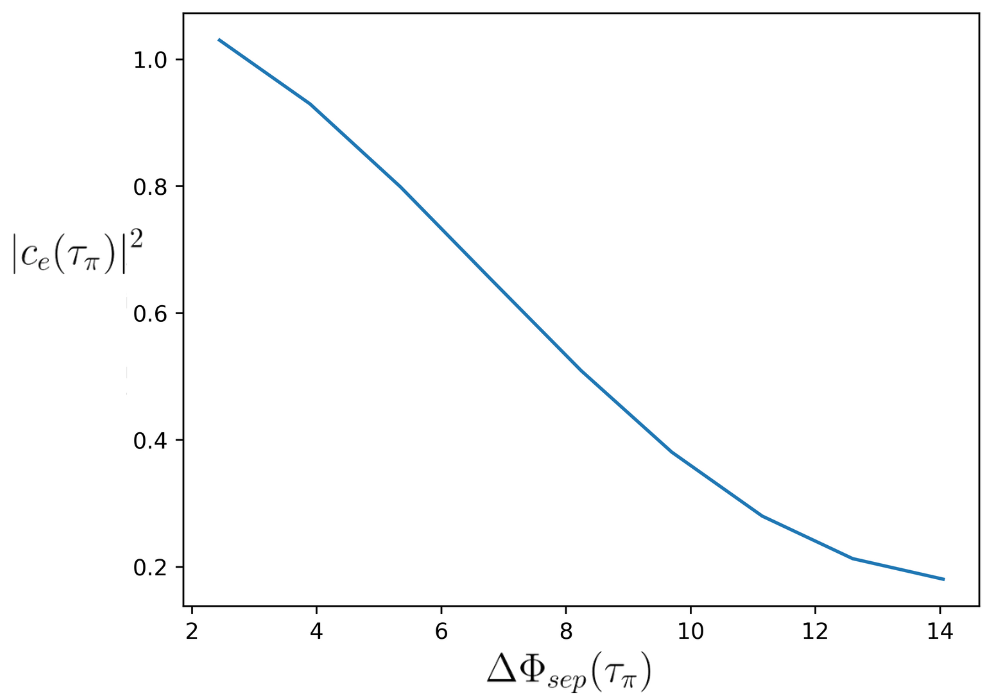
\includegraphics[width=0.7\textwidth]{decoherence rabi oscillations.png}
\caption{Phase shift due to the finite duration of a $\pi$-pulse used to drive Rabi oscillations (Eq. \ref{phaseshiftpos}) versus the population of the excited state immediately after the pulse is applied. All the population is initially in the ground state, thus, full visibility means that after the pulse is applied all the population is transferred to the excited state. Notice that when the phase shift is of the order of $\pi$, the visibility is reduced significantly, this establishes the condition in Eq. \ref{condpower}.}
\label{decoherence_rabi_oscillations_plot}
\end{figure}

In this section, we will provide a heuristic proof of the condition in Eq. \ref{condpower} through a numerical simulation. The sequence of pulses of Eq. \ref{pulses} is applied to a cloud of atoms in free-fall. Thus, since the duration of the pulses is finite, during the process of Rabi oscillations, every atom not only undergoes a change in its internal state but also a change in its external state. Let's suppose that the atom is initially in the ground state ($g$) and has a moment $p$ such that it can be described by $\ket{\psi(0)} = \ket{g, p}$. To make this state evolve, we will apply an algorithm similar to the split-operator method used in Section \ref{split_op_method_section}. We will consider infinitesimal steps in time and at every step, the state will evolve first in momentum and then in its internal state through the Rabi oscillations.

The change in momentum due to an infinitesimal step in time for an atom under a free-fall Hamiltonian (Eq. \ref{free_fall_hamiltonian}) was calculated in Eq. \ref{small_step_momentum_eq}. On the other hand, the most general solution to the Rabi oscillations is given by \cite{sakurai2017modern}

\begin{equation}
    \begin{aligned}
        C_{g}(t) & = C_{g}(0) \cos{\frac{\Omega t}{2}} - i  C_{e}(0) \sin{\frac{\Omega t}{2}}, \\ C_{e}(t) &= C_{e}(0) \cos{\frac{\Omega t}{2}} - i  C_{g}(0) \sin{\frac{\Omega t}{2}}.
    \end{aligned}
\end{equation}
%
For infinitesimal small time steps, this solution can be approximated as

\begin{equation}\label{rabi_small_step_solution_eq}
    \begin{aligned}
        C_{g}(t) & \approx C_{g}(0) - i  C_{e}(0) \frac{\Omega t}{2}, \\ C_{e}(t) &\approx C_{e}(0) - i  C_{g}(0) \frac{\Omega t}{2}.
    \end{aligned}
\end{equation}
%
Therefore, we can use Eqs. \ref{small_step_momentum_eq} and \ref{rabi_small_step_solution_eq} to compute the evolution at every time step. For the first time step, the change in momentum applied to the initial state ($\ket{\psi (0)} = \ket{g, p}$) gives

\begin{equation*}
    \ket{\psi (\Delta t)} = \exp \bigg( -\frac{i}{\hbar} \frac{(p-\hbar \Delta k_{-})^{2}}{2m} \Delta t \bigg)\ket{g, p-\hbar \Delta k_{-}},
\end{equation*}
%
by applying the Rabi oscillations on this state gives

\begin{multline*}
    \ket{\psi (\Delta t)} = \exp \bigg( -\frac{i}{\hbar} \frac{(p-\hbar \Delta k_{-})^{2}}{2m} \Delta t \bigg)\ket{g, p-\hbar \Delta k_{-}}
    \\ - i \frac{\Omega t}{2} \exp \bigg( -\frac{i}{\hbar} \frac{(p-\hbar \Delta k_{-})^{2}}{2m} \Delta t \bigg)\ket{e, p-\hbar \Delta k_{-}},
\end{multline*}
%
Notice that we have defined

\begin{equation}
    k_{\pm} \equiv \frac{m a_{\pm}}{\hbar} t,
\end{equation}
%
to distinguish between the momentum transferred in the excited state from that transferred in the ground state (see Eq. \ref{a1a2}). For the second time step, the change in momentum produces

\begin{multline*}
    \ket{\psi (2 \Delta t)}= \exp \bigg( -\frac{i}{\hbar} \frac{(p-\hbar \Delta k_{-})^{2} + (p-2\hbar \Delta k_{-})^{2}}{2m} \Delta t \bigg)\ket{g, p-2\hbar \Delta k_{-}}
    \\ - i \frac{\Omega t}{2} \exp \bigg( -\frac{i}{\hbar} \frac{(p-\hbar \Delta k_{-})^{2} + (p-\hbar \Delta k_{-} -\hbar \Delta k_{+})^{2}}{2m} \Delta t \bigg)\ket{e, p-\hbar \Delta k_{-} -\hbar \Delta k_{+}},
\end{multline*}
%
while the Rabi oscillations produce

\begin{multline*}
    \ket{\psi (2 \Delta t)} = \exp \bigg( -\frac{i}{\hbar} \frac{(p-\hbar \Delta k_{-})^{2} + (p-2\hbar \Delta k_{-})^{2}}{2m} \Delta t \bigg)\ket{g, p-2\hbar \Delta k_{-}}
    \\ - i \frac{\Omega t}{2} \exp \bigg( -\frac{i}{\hbar} \frac{(p-\hbar \Delta k_{-})^{2} + (p-2\hbar \Delta k_{-})^{2}}{2m} \Delta t \bigg)\ket{e, p-2\hbar \Delta k_{-}}
    \\ - i \frac{\Omega t}{2} \exp \bigg( -\frac{i}{\hbar} \frac{(p-\hbar \Delta k_{-})^{2} + (p-\hbar \Delta k_{-} -\hbar \Delta k_{+})^{2}}{2m} \Delta t \bigg)\ket{e, p-\hbar \Delta k_{-} -\hbar \Delta k_{+}}
    \\ - \bigg(\frac{\Omega t}{2}\bigg)^2 \exp \bigg( -\frac{i}{\hbar} \frac{(p-\hbar \Delta k_{-})^{2} + (p-\hbar \Delta k_{-} -\hbar \Delta k_{+})^{2}}{2m} \Delta t \bigg)\ket{g, p-\hbar \Delta k_{-} -\hbar \Delta k_{+}}.
\end{multline*}
%
For the third iteration, we follow the same procedure, and so on. Notice that the algorithm becomes computationally more expensive at each iteration, therefore, the procedure must be stopped after N time steps, and the amplitude of all the sub-states that ended up in the ground (excited) state can be summed to compute the global amplitude of the ground (excited) state and from this, the final population of the corresponding state can be inferred. The following program performs several simulations of this algorithm with different initial velocities (corresponding to different initial cloud temperatures \cite{edgarMagneticGravimeter}). For each simulation, the phase shift of Eq. \ref{phaseshiftpos} is computed and recorded as well. Finally, the phase shift due to the finite pulse duration obtained at each iteration is plotted against the corresponding visibility of the Rabi oscillations obtained through the simulation. The output of the program is shown in Fig. \ref{decoherence_rabi_oscillations_plot}. By looking at this plot, the condition of Eq. \ref{condpower} is obtained.
\\
\begin{lstlisting}[language=Python, caption=Python code for the simulation of decoherence of the Rabi oscillations in a magnetic gravimeter.]
import numpy as np
import matplotlib.pyplot as plt

num_experiments = 10  # Number of simulations
rabi_steps = 26  # Number of Rabi oscillation steps

# Constants
hbar = 1e-34
m = 1e-25  # Mass of 87Rb
g = 9.8  # Gravitational acceleration
w = 1e4  # Rabi frequency
initial_velocity = 3e-3  # Initial velocity

# Parameters
magnetic_acceleration = g / 6  # Magnetic acceleration
g1 = g + magnetic_acceleration  # Acceleration 1
g2 = g - magnetic_acceleration  # Acceleration 2
t_pi = np.pi / w  # Time for a pi pulse
dt = t_pi / rabi_steps  # Time step
iw_dt_2 = -1j * w * dt / 2  # Factor for Rabi oscillations
fp = -1j * dt / (2 * m * hbar)  # Factor for temporal evolution
dp1 = m * g1 * dt  # Momentum change with g1
dp2 = m * g2 * dt  # Momentum change with g2

# Global results
cef_squared_values = []
phase_values = []

# perform simulation several times
for it in range(1, num_experiments):
    v = it * initial_velocity
    p = m * v  # Initial momentum

    phase = (m / (2 * hbar)) * (3 * v * (g1 - g2) * (t_pi ** 2) + ((g1 ** 2) - (g2 ** 2)) * (t_pi ** 3))
    phase_values.append(phase)

    pgv = np.array([p])
    pev = np.array([p])

    # begin with all population in ground state
    cgv = np.array([1 + 0j])  # Initial coefficient g
    cev = np.array([0 + 0j])  # Initial coefficient e

    time_values = np.array([0])
    cef = [cev[0]]
    cgf = [cgv[0]]

    # compute rabi oscillation for rabi_steps
    for step in range(rabi_steps):
        time_values = np.append(time_values, time_values[-1] + dt)
        pgv = np.append(pgv, pgv[-1] + dp1)
        pev = np.append(pev, pev[-1] + (dp1 if step == 0 else dp2))

        # Apply temporal evolution only to relevant elements
        cgv *= np.exp(fp * (pgv[-1] ** 2))
        cev *= np.exp(fp * (pev[-1] ** 2))

        # Rabi oscillations, doubling the number of components
        cgv_temp = np.concatenate([cgv, iw_dt_2 * cev])
        cev_temp = np.concatenate([cev, iw_dt_2 * cgv])
        cgv, cev = cgv_temp, cev_temp

        # Double the size of pgv and pev to match cgv and cev
        pgv = np.concatenate([pgv, np.full(len(cgv) - len(pgv), pgv[-1])])
        pev = np.concatenate([pev, np.full(len(cev) - len(pev), pev[-1])])

        # Update the final coefficients
        cgf.append(np.sum(cgv))
        cef.append(np.sum(cev))

        # Add a new time value only after completing all operations
        time_values = np.append(time_values, time_values[-1] + dt)

    # Ensure that time_values and cef have the same length
    time_values = time_values[:len(cef)]

    cef_squared = np.abs(cef) ** 2

    # Plot (adjust according to reference data)
    plt.plot(time_values, cef_squared)
    plt.xlabel('time (s)')
    plt.ylabel('|c_e|^2')
    plt.text(t_pi / 10, 0.6, f'phase: {phase}')
    plt.pause(0.3)

    cef_squared_values.append(cef_squared[-1])

# Final plot
plt.figure()
plt.plot(phase_values, cef_squared_values)
plt.xlabel('phase')
plt.ylabel('|c_e(t=t_pi)|^2')
plt.show()
\end{lstlisting}


\bibliographystyle{plain}
\bibliography{cites.bib}

\end{document}